%%%% documentation_sentinelle.tex
%%%% Data Challenge Burkina 2026, édition Éducation, défi 1 : documentation de la solution (15 pages au plus).
%%%% Mise en page reprise du gabarit de la note d'intention. Évaluation anonyme : aucun nom, aucune affiliation.
%%%% Compilation : tectonic documentation_sentinelle.tex (ou pdflatex puis bibtex). Figures : python figures.py.

\documentclass{article}

\usepackage{ijcai26}

\usepackage{times}
\usepackage{url}
\usepackage[utf8]{inputenc}
\usepackage[T1]{fontenc}
\usepackage[english,french]{babel}
\usepackage{xcolor}
\usepackage{xurl}
\usepackage[colorlinks=true,
            citecolor=blue!70!black,
            linkcolor=red!60!black,
            urlcolor=blue!70!black,
            pdfauthor={},
            pdftitle={Sentinelle Scolaire : documentation de la solution},
            pdfcreator={},
            pdfproducer={}]{hyperref}
\usepackage[small]{caption}
\usepackage{graphicx}
\usepackage{amsmath}
\usepackage{booktabs}
\usepackage{tabularx}
\usepackage{array}
\usepackage{float}
\usepackage{placeins}

\urlstyle{same}
\renewcommand{\topfraction}{0.92}
\renewcommand{\dbltopfraction}{0.92}
\renewcommand{\bottomfraction}{0.6}
\renewcommand{\textfraction}{0.06}
\renewcommand{\floatpagefraction}{0.85}
\renewcommand{\dblfloatpagefraction}{0.85}
\setcounter{topnumber}{4}
\setcounter{dbltopnumber}{3}
\setcounter{totalnumber}{6}
\emergencystretch=1.5em
\graphicspath{{figures/}}

\addto\captionsfrench{%
  \renewcommand{\tablename}{Tableau}%
  \renewcommand{\figurename}{Figure}%
  \renewcommand{\refname}{Références}%
}

\newcommand{\sol}{Sentinelle Scolaire}
\newcommand{\lien}{\url{https://sentinelle-scolaire-bf.up.railway.app}}
\newcolumntype{L}[1]{>{\raggedright\arraybackslash}p{#1}}
\newcolumntype{Y}{>{\raggedright\arraybackslash}X}

\title{\sol{}\\[3pt]
{\large\mdseries Cartographier et anticiper le risque de décrochage scolaire au primaire, province par province}}
\author{
Data Challenge Burkina 2026, édition Éducation, défi 1\\
\affiliations
Documentation de la solution \\
Application en ligne : \lien
}

\begin{document}
\renewcommand{\tablename}{Tableau}\renewcommand{\figurename}{Figure}\renewcommand{\refname}{Références}
\raggedbottom

\maketitle
\thispagestyle{plain}
\pagestyle{plain}

\begin{abstract}
\sol{} est un outil d'aide à la décision qui dit où le décrochage au primaire risque d'être le plus fort au Burkina Faso, pourquoi, et comment l'anticiper. À partir des annuaires de la DGESS, des données de l'INSD, des rapports du ST-ESU et des déplacés internes, nous avons construit un panel de 47 provinces (découpage de 2025) sur neuf années scolaires. Dix modèles de prévision ont été comparés dans le temps, sur des années jamais vues : le modèle retenu, un retour amorti vers le niveau habituel de chaque province, prévoit le taux d'abandon avec une erreur moyenne de 3,3 points, contre 4,4 pour la méthode naïve, et donne un intervalle à 80 \% dont la couverture mesurée va de 85 à 94 \%. Les prévisions vont jusqu'en 2027-2028. Une alerte distincte repère les ruptures de scolarisation (AUC de 0,85 à 0,96), et les valeurs SHAP expliquent chaque province. Pour 2025-2026, le taux national prévu est de 8,0 \%, soit environ 266\,000 élèves ; 12 provinces sont en risque élevé et 11 en alerte de rupture, surtout dans le nord et l'est. L'outil est en ligne : carte, fiches, simulateur, mise à jour annuelle sans réentraînement, assistant et rapports PDF.
\end{abstract}

%======================================================================
\section{Le défi}
%======================================================================

\textbf{La question.} Le défi 1 demande où le risque de décrochage scolaire est le plus fort, par région, et comment l'anticiper~\cite{dcb_document}. Nous la reformulons ainsi : \emph{pour chaque province, quel sera le taux d'abandon du primaire l'an prochain et les deux années suivantes, avec quelle incertitude, qu'est-ce qui l'explique, et où une rupture brutale de la scolarisation menace-t-elle ?}

\textbf{Pourquoi c'est urgent.} En 2024-2025, le taux d'achèvement du primaire n'est que de 51,6 \% : sur deux enfants qui entrent au CP1, un seul atteint la fin du CM2~\cite{dgess_base}. Les écarts entre régions vont de un à huit, et les régions les plus touchées par la crise sécuritaire cumulent fermetures d'écoles et déplacements de population~\cite{stesu,conasur}. Le système ne mesure l'abandon qu'après coup, dans l'annuaire de l'année suivante.

\textbf{Pour qui.} Le ministère et ses directions régionales et provinciales, qui doivent répartir des moyens limités (enseignants, cantines, places assises, programmes de seconde chance) et préparer la continuité éducative là où des écoles risquent de fermer.

\textbf{Notre réponse.} Une chaîne complète, des données brutes à la décision, en cinq étapes (figure~\ref{fig:parcours}) : un modèle de prévision évalué honnêtement, une explication province par province, une alerte de rupture, et un tableau de bord en ligne qui transforme ces résultats en actions.

\begin{figure*}[!t]
\centering
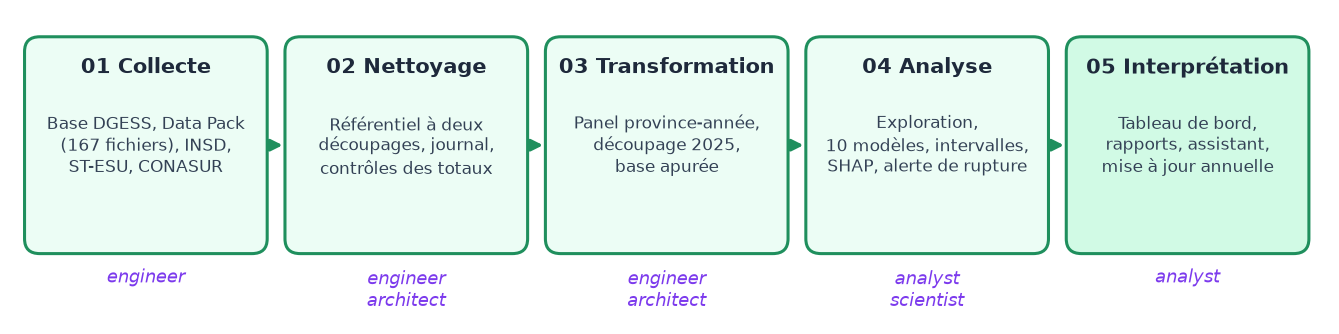
\includegraphics[width=0.92\textwidth]{fig_parcours}
\caption{Parcours des données de \sol{}, des sources à la décision, et rôles qui portent chaque étape. Chaque étape est un module Python présenté par un notebook exécuté et produit son dépôt.}
\label{fig:parcours}
\end{figure*}

%======================================================================
\section{Les données}
%======================================================================

\textbf{Sources.} Toutes les données proviennent des fichiers remis par les organisateurs : la base principale de la DGESS~\cite{dgess_base} et le Data Pack de 167 fichiers~\cite{dcb_guide}, complétés par trois annuaires régionaux de l'INSD absents du pack~\cite{insd_annuaires}. Sur 347 fichiers remis, 118 sont retenus et répartis en 33 jeux de données ; chacun des 55 fichiers écartés l'est pour un motif écrit (hors du champ du primaire, géométries, doublons). Le tableau~\ref{tab:sources} résume ce que chaque source apporte.

\begin{table}[!t]
\centering
\footnotesize
\begin{tabularx}{\columnwidth}{@{}L{2.75cm} Y L{1.15cm}@{}}
\toprule
Source & Apport & Niveau \\
\midrule
Annuaires du primaire DGESS (8 éditions)~\cite{dgess_annuaires} & Taux d'abandon, de redoublement et de promotion (cible), effectifs, maîtres, salles, équipement, distance & Province \\
Base principale DGESS~\cite{dgess_base} & Admission, scolarisation, achèvement, CEP, parité ; contrôle des totaux & Région \\
Annuaires post-primaire et secondaire, tableaux de bord DGESS~\cite{dgess_pps,dgess_tdb} & Admission en 6e, achèvement, abandon au post-primaire ; séries régionales, causes d'abandon & Province, région \\
RGPH 2019, INSD~\cite{insd_rgph,insd_pauvrete} & Pauvreté, enfants hors de l'école, travail des enfants, mariage précoce, alphabétisation & Commune \\
ST-ESU~\cite{stesu} & Écoles fermées et rouvertes, élèves concernés & Région, province \\
CONASUR~\cite{conasur} & Déplacés internes et enfants déplacés & Commune \\
Projections de population, INSD~\cite{insd_projections} & Population par âge simple et sexe, 2020-2035 & Commune, province \\
COD-AB~\cite{codab}, OpenStreetMap~\cite{hotosm} & 351 communes, anciens et nouveaux codes, contours ; noms des localités & Commune \\
\bottomrule
\end{tabularx}
\caption{Principales sources. Le registre des sources (dépôt 01) donne pour chaque fichier son adresse d'origine et son empreinte SHA-256.}
\label{tab:sources}
\end{table}

\textbf{Unité d'analyse.} La province, dans le découpage de juillet 2025 (17 régions, 47 provinces), sur neuf années scolaires (2016-2017 à 2024-2025), soit 423 lignes pour l'ensemble des élèves et 846 pour les filles et les garçons. La cible est le taux d'abandon du primaire publié par la DGESS ; le taux de l'année $t$ est mesuré entre $t-1$ et $t$.

\begin{table}[!t]
\centering
\footnotesize
\begin{tabularx}{\columnwidth}{@{}L{2.25cm} Y@{}}
\toprule
Famille & Exemples de variables (valeur connue en $t$) \\
\midrule
Passé scolaire & abandon et redoublement de l'année, poids du CP1, rapport CM2/CP1, réussite au CEP \\
Effectifs & élèves du primaire, évolution, ruptures passées, part des filles \\
Encadrement et offre & élèves par maître et par salle, enseignantes, enseignants débutants, places assises manquantes, manuels, logements de maîtres \\
Équipement des écoles & eau potable, électricité, latrines, cantines, écoles à cycle incomplet, salles précaires \\
Accès et âge & élèves à plus de 3 km, entrée tardive au CP1, élèves de 12 ans et plus \\
Post-primaire & admission en 6e, scolarisation, achèvement, abandon au post-primaire \\
Contexte social (RGPH 2019) & pauvreté, enfants hors de l'école, jeunes ni à l'école ni en emploi, travail des enfants, filles mariées à 17 ans, alphabétisation \\
Contexte régional & parités, préscolarisation, écoles privées, abandons pour orpaillage, mariage ou grossesse \\
\bottomrule
\end{tabularx}
\caption{Familles de variables de la table d'analyse (79 colonnes). Le dictionnaire des variables (dépôt 03) donne pour chacune sa description, son unité, sa source et sa part de valeurs manquantes.}
\label{tab:familles}
\end{table}

\textbf{Variables.} Le tableau~\ref{tab:familles} présente les familles de variables. Toutes portent sur l'année $t$ ou les précédentes : aucune information du futur n'entre dans la prévision.

\textbf{Limites connues.} Trois limites sont signalées dans les dépôts et prises en compte par le modèle. (1) La répartition filles-garçons des effectifs de 2024-2025 est invraisemblable pour 31 provinces : seul le total est utilisé pour cette année. (2) Les rapports du ST-ESU, lus dans des PDF, ne sont fiables qu'au niveau régional, et ne recensent plus les fermetures à partir d'octobre 2023. (3) Les années de crise produisent des variations d'effectifs de plus de 30 \% (fermetures massives) : ces \emph{ruptures} concernent 8 \% des lignes mais 73 \% de la variance du taux d'abandon. Elles sont traitées à part (section~\ref{sec:methode}).

%======================================================================
\section{La préparation}
%======================================================================

La collecte et le nettoyage sont décrits en détail dans deux documents techniques déposés avec les étapes 02 et 03 ; nous en donnons ici l'essentiel.

\textbf{Collecte (dépôt 01).} Un catalogue déclaratif indique, pour chaque jeu, les fichiers, les pages et les tableaux à extraire. Les lignes sont copiées sans modification et gardent leur fichier, leur page et leur ligne d'origine. Les fichiers des organisateurs restent en lecture seule : le code refuse d'écrire dans leur dossier.

\textbf{Nettoyage (dépôt 02).} Trois pièges signalés par le challenge ont été traités. \emph{Les noms de provinces} s'écrivent de plusieurs façons : une table d'alias les ramène à un code unique. \emph{Les anciennes et nouvelles régions} ne se recoupent pas : le référentiel part de la commune, qui porte à la fois son code de l'ancien découpage (13 régions, 45 provinces), utilisé par toutes les données de la DGESS, et celui de 2025. \emph{L'année scolaire} n'est pas l'année civile : toutes les tables sont indexées par année scolaire. Chaque correction est consignée dans un journal (valeur avant, valeur après, motif), et des contrôles automatiques comparent la somme des provinces aux totaux régionaux et nationaux publiés.

\textbf{Transformation (dépôt 03).} Le panel province-année réunit la cible et 79 variables connues à la date $t$ : passé scolaire, effectifs, encadrement, équipement, contexte social du RGPH 2019, exposition à la crise. Le passage au découpage de 2025 répartit les effectifs des deux provinces scindées (Soum et Tapoa) selon des clés communales de l'INSD. La \emph{base apurée} ne contient aucune cellule vide : les valeurs impossibles sont recodées, les manquants imputés par une méthode choisie par test, et le statut de chaque cellule (observée, valeur publiée de l'INSD, imputée) est conservé. Règle centrale : \textbf{seules les cibles observées servent à entraîner et à évaluer les modèles}.

\begin{table}[!t]
\centering
\footnotesize
\begin{tabularx}{\columnwidth}{@{}Y r@{}}
\toprule
Contrôle ou statut & Résultat \\
\midrule
Provinces présentes chaque année (flux, effectifs) & 45 sur 45 \\
Garçons + filles = total & 0 écart \\
Abandon + redoublement + promotion = 100 & 423 lignes sur 423 \\
Somme des provinces = total régional publié & 98,8 \% des 3\,236 comparaisons \\
Corrections consignées dans le journal & 2\,410 \\
\midrule
Cellules de la base apurée observées & 87,7 \% \\
Imputées (méthode choisie par test) & 6,0 \% \\
Complétées par le passage à 2025 & 5,1 \% \\
Valeurs publiées par l'INSD & 1,2 \% \\
\bottomrule
\end{tabularx}
\caption{Qualité de la préparation : contrôles automatiques et statut des 29\,187 cellules de la base apurée. Les écarts aux totaux publiés sont listés un par un dans les dépôts 02 et 03.}
\label{tab:qualite}
\end{table}

Le tableau~\ref{tab:qualite} chiffre la qualité obtenue : près de neuf cellules sur dix sont des valeurs observées, et aucune valeur observée n'a été modifiée par l'apurement (25\,595 cellules comparées, aucun écart).

%======================================================================
\section{La méthode et son évaluation}
\label{sec:methode}
%======================================================================

\subsection{Ce que révèle l'exploration}

Avant tout modèle, l'analyse exploratoire (notebook \texttt{04a}) a établi trois faits qui guident toute la méthode.

\textbf{Les ruptures dominent la variance.} Avec les années de rupture, la variance du taux d'abandon est de 237 points$^2$ ; sans elles, de 63 : les ruptures, 8 \% des lignes, portent près des trois quarts de la variance. Un modèle unique serait dominé par quelques années de crise ; d'où la séparation entre abandon et rupture.

\textbf{Le décrochage est persistant.} Hors ruptures, 37 \% de la variance oppose les provinces entre elles, et la moyenne passée d'une province prévoit mieux l'année suivante (erreur de 4,7 points) que le taux de l'année (5,7) ou la médiane des provinces (5,3). Le niveau habituel est donc la référence naturelle à battre.

\textbf{Une variable sur deux est redondante.} Sur 69 variables candidates, 35 sont gardées et 34 retirées, chacune pour un motif écrit : colinéarité ($|\rho| \geq 0{,}85$, on garde la plus observée ou la plus liée à la cible), redondance linéaire (facteur d'inflation de la variance supérieur à 10), lien faible et instable dans le temps, trop peu de valeurs observées, ou identité comptable (figure~\ref{fig:decisions}).

\begin{figure}[!htbp]
\centering
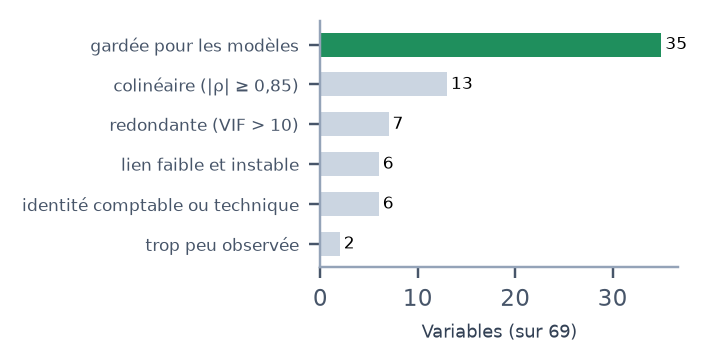
\includegraphics[width=0.62\columnwidth]{fig_decisions_variables}
\caption{Décision motivée pour chacune des 69 variables candidates (ensemble des élèves).}
\label{fig:decisions}
\end{figure}

\subsection{Trois briques}

\textbf{Brique 1, prévision.} Le taux d'abandon est transformé en $z = \mathrm{logit}(\text{taux}/100)$ avant modélisation, puis ramené en pourcentage : les prévisions et les intervalles restent entre 0 et 100 \% et deviennent asymétriques, comme les taux eux-mêmes. Dix modèles sont comparés : trois références (taux de l'année précédente, niveau habituel de la province, niveau rétréci vers la région), quatre modèles appris (elastic net~\cite{elasticnet}, ridge avec effet province, LightGBM~\cite{lightgbm}, LightGBM après élimination récursive guidée par SHAP), et trois combinaisons. Le \emph{niveau habituel} est la moyenne des taux passés de la province, années de rupture exclues. Le \emph{retour amorti} part de ce niveau et laisse l'écart de la dernière année se résorber d'un facteur $\varphi$ par an~\cite{hyndman} :
\begin{equation}
z_{t+h} = \bar z_p + \varphi^{h}\,(z_t - \bar z_p),
\end{equation}
où $\bar z_p$ est le niveau habituel de la province $p$ et $h$ l'horizon (1 à 3 ans). La sélection des variables (importance par permutation, élimination guidée par SHAP) et le choix des réglages ($\varphi$, pénalités, profondeur des arbres) sont refaits dans chaque pli, sur la seule information de l'apprentissage : aucune fuite du futur.

\textbf{Intervalle.} Un intervalle conforme à 80 \%~\cite{vovk,angelopoulos} est calculé sur l'échelle logit à partir des erreurs hors échantillon, puis dénormalisé. Sa marge ne diminue jamais avec l'horizon : à trois ans, l'incertitude est au moins celle de deux ans.

\textbf{Brique 2, explication.} Pourquoi une province a-t-elle un niveau habituel élevé ? Deux modèles sont validés en prédisant des provinces qu'ils n'ont pas vues (validation croisée par groupes de provinces) : un elastic net donne l'effet chiffré de cinq variables (utilisé par le simulateur), et un LightGBM réduit à huit variables par élimination récursive donne, par les valeurs SHAP~\cite{shap}, la contribution de chaque variable au niveau de chaque province. Les variables de persistance (taux passés) sont exclues : expliquer le niveau par le niveau serait circulaire.

\textbf{Brique 3, alerte de rupture.} Une régression logistique pénalisée, aux classes équilibrées, estime le risque qu'une province voie ses effectifs varier de plus de 30 \% l'année suivante, à partir de sept signaux connus à l'avance : évolution et baisse des effectifs, ruptures passées, abandon de l'année, abandons pour orpaillage, jeunes hors de l'école.

\subsection{Un protocole d'évaluation sans complaisance}

Les modèles sont évalués \emph{dans le temps} : on apprend sur les années passées et on prévoit l'année suivante, sur trois plis de sélection (cibles 2021-2022 à 2023-2024), puis sur un \textbf{test final}, 2024-2025, qui n'a jamais servi à choisir quoi que ce soit. Trois mesures, en points de taux après dénormalisation : l'erreur absolue moyenne, la corrélation de rang entre taux prévus et observés, et le rappel du quintile le plus à risque (part des provinces réellement les plus touchées que la prévision retrouve).

\textbf{Règle de choix, fixée avant de regarder le test.} Le niveau habituel est le modèle à battre. Un autre modèle n'est retenu que s'il réduit l'erreur des plis de sélection d'au moins 3 \% \emph{et} fait mieux sur au moins deux plis sur trois : un écart plus faible s'explique par le hasard des plis. À défaut, un modèle qui suit la situation de l'année (retour amorti, combinaison) est préféré s'il est aussi précis, à 1 \% près.

\subsection{Résultats de l'évaluation}

\begin{figure}[!htbp]
\centering
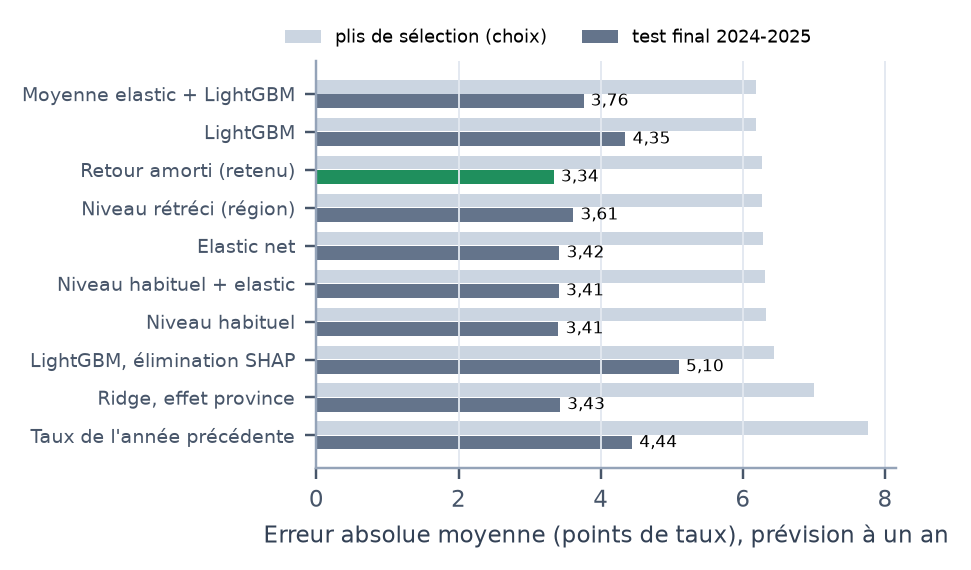
\includegraphics[width=\columnwidth]{fig_comparaison_modeles}
\caption{Erreur des dix modèles à un an, sur les plis de sélection (choix) et sur le test final 2024-2025 (jamais vu). Ensemble des élèves.}
\label{fig:modeles}
\end{figure}

\textbf{Aucun modèle appris ne bat durablement le niveau habituel} (figure~\ref{fig:modeles}). Les modèles appris gagnent un peu les années de crise et perdent les années calmes : les variables provinciales ne prévoient pas bien les chocs d'une année sur l'autre, qui sont surtout communs à tout le pays. Le décrochage est \emph{structurel et persistant}. C'est un résultat en soi, et nous le présentons tel quel plutôt que de retenir un modèle plus complexe sur la foi d'un seul test.

\begin{table}[!t]
\centering
\footnotesize
\begin{tabular}{@{}l r r r r@{}}
\toprule
& Sélection & \multicolumn{3}{c}{Test final 2024-2025} \\
Modèle & 1 an & 1 an & 2 ans & 3 ans \\
\midrule
LightGBM & 6,18 & 4,35 & 3,52 & 3,28 \\
Moyenne elastic net + LightGBM & 6,18 & 3,76 & 3,45 & 3,04 \\
Niveau rétréci vers la région & 6,27 & 3,61 & 3,78 & 3,21 \\
\textbf{Retour amorti (retenu)} & \textbf{6,27} & \textbf{3,34} & \textbf{3,67} & \textbf{3,01} \\
Elastic net & 6,29 & 3,42 & 3,61 & 3,03 \\
Niveau habituel + elastic net & 6,31 & 3,41 & 3,58 & 3,02 \\
Niveau habituel (référence) & 6,32 & 3,41 & 3,55 & 3,01 \\
LightGBM après élimination SHAP & 6,43 & 5,10 & 4,68 & 3,36 \\
Ridge avec effet province & 7,00 & 3,43 & 4,80 & 2,94 \\
Taux de l'année précédente & 7,77 & 4,44 & 15,15 & 10,62 \\
\bottomrule
\end{tabular}
\caption{Erreur absolue moyenne (points de taux) des dix modèles, ensemble des élèves. Les plis de sélection servent au choix, le test final à la mesure.}
\label{tab:dixmodeles}
\end{table}

\textbf{La règle a évité un piège.} Sur les plis de sélection, LightGBM avait la plus faible erreur (6,18), mais seulement 2,2 \% sous le niveau habituel, en dessous des 3 \% exigés. Au test, il tombe à 4,35 points, contre 3,34 pour le modèle retenu (tableau~\ref{tab:dixmodeles}) : il n'était meilleur que par le hasard des plis. Une règle fixée à l'avance protège de ce genre d'illusion.

Le \textbf{retour amorti} ($\varphi = 0{,}2$ pour l'ensemble, $0{,}3$ par sexe) est aussi précis que le niveau habituel sur les plis de sélection (6,27 contre 6,32 points) et il est retenu par la règle. Au test final, son erreur est de \textbf{3,34 points à un an} contre 3,41 pour le niveau habituel et \textbf{4,44 pour la méthode naïve} (reconduire le taux de l'année) ; à deux et trois ans, elle est de 3,67 et 3,01 points (tableau~\ref{tab:fiabilite}). Il retrouve 75 \% des provinces du quintile le plus à risque. Par sexe, l'erreur au test est de 4,15 points à un an et de 3,61 à deux ans.

\begin{table}[!t]
\centering
\footnotesize
\begin{tabularx}{\columnwidth}{@{}Y r r r@{}}
\toprule
Mesure (test final 2024-2025) & 1 an & 2 ans & 3 ans \\
\midrule
Erreur, retour amorti (points) & 3,34 & 3,67 & 3,01 \\
Erreur, niveau habituel & 3,41 & 3,55 & 3,01 \\
Erreur, taux de l'année précédente & 4,44 & 15,15 & 10,62 \\
Rappel du quintile le plus à risque & 0,75 & 0,62 & 0,75 \\
Couverture de l'intervalle à 80 \% & 85 \% & 88 \% & 85 \% \\
Couverture, par sexe & 86 \% & 94 \% & 92 \% \\
\bottomrule
\end{tabularx}
\caption{Fiabilité de la prévision au test final, ensemble des élèves (40 provinces à cible observée hors rupture), sauf dernière ligne.}
\label{tab:fiabilite}
\end{table}

\begin{figure}[!htbp]
\centering
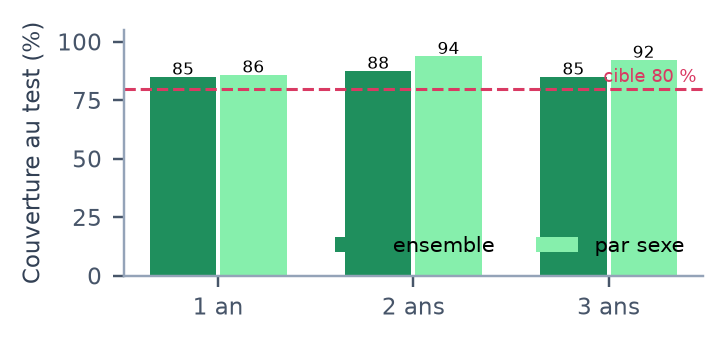
\includegraphics[width=0.96\columnwidth]{fig_couverture}
\caption{Couverture de l'intervalle à 80 \% au test final : la part des taux réels tombés dans l'intervalle annoncé dépasse la cible à tous les horizons.}
\label{fig:couverture}
\end{figure}

\textbf{L'intervalle tient sa promesse} : 85 à 88 \% des taux réels tombent dans l'intervalle annoncé à 80 \% (figure~\ref{fig:couverture}). Sa largeur moyenne, 18 à 20 points, est le prix honnête de la volatilité des taux provinciaux : la classe de risque est plus fiable que le chiffre exact, et c'est elle que le tableau de bord met en avant.

\begin{figure}[!htbp]
\centering
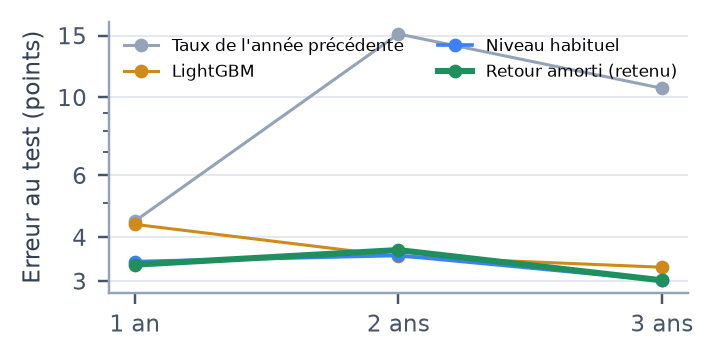
\includegraphics[width=\columnwidth]{fig_erreur_horizon}
\caption{Erreur au test final selon l'horizon (échelle logarithmique) : reconduire le taux de l'année devient très coûteux à deux et trois ans, alors que le retour amorti reste stable.}
\label{fig:horizon}
\end{figure}

\textbf{La prévision tient à trois ans.} Reconduire le taux de l'année, comme on le fait souvent faute de mieux, coûte 15 points d'erreur à deux ans ; le retour amorti reste autour de 3 points à tous les horizons (figure~\ref{fig:horizon}). C'est ce qui justifie des projections jusqu'en 2027-2028, et pas au-delà.

\textbf{Par sexe}, le même protocole donne une erreur au test de 4,15 points à un an et de 3,61 à deux ans, contre 8,72 et 5,32 pour la méthode naïve ; le retour amorti est retenu avec $\varphi = 0{,}3$. Le modèle par sexe garde une variable « fille » et des variables publiées par sexe (flux, effectifs, âges), ancrées sur l'ensemble pour que filles et garçons redonnent le total.

\textbf{L'explication se généralise} à des provinces non vues : l'elastic net explique 64 \% des écarts entre provinces, le LightGBM réduit 52 \% (47 et 45 \% par sexe). \textbf{L'alerte de rupture discrimine bien} : AUC de 0,87, 0,85 et 0,91 sur les plis de sélection et de \textbf{0,96 au test final} ; au test, les deux ruptures de l'année figurent dans le quart des provinces au score le plus élevé (figure~\ref{fig:auc}). Les signaux qui comptent le plus sont la part de jeunes de 16 à 18 ans hors de l'école, l'abandon de l'année et les ruptures passées ; une baisse récente des effectifs, déjà absorbée, réduit le risque d'une nouvelle rupture (figure~\ref{fig:signaux}).

\begin{figure}[!htbp]
\centering
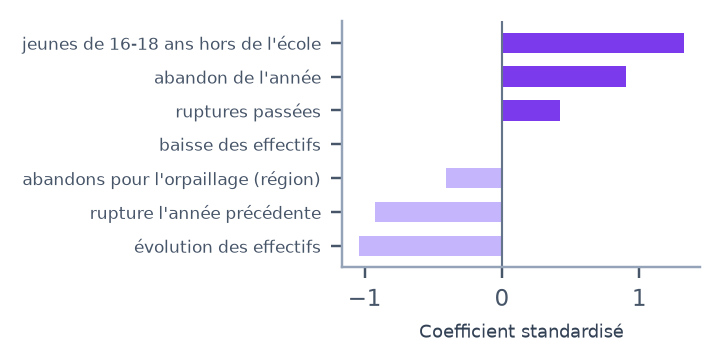
\includegraphics[width=0.66\columnwidth]{fig_signaux_alerte}
\caption{Signaux de l'alerte de rupture (coefficients standardisés de la régression logistique).}
\label{fig:signaux}
\end{figure}

\begin{figure}[!htbp]
\centering
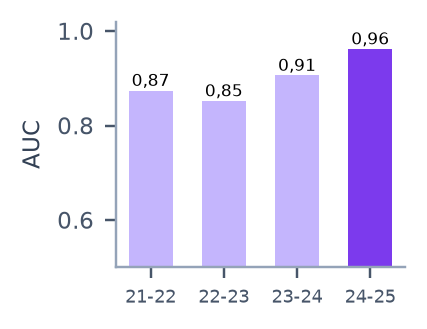
\includegraphics[width=0.55\columnwidth]{fig_alerte_auc}
\caption{AUC de l'alerte de rupture par année cible (foncé : test final).}
\label{fig:auc}
\end{figure}

%======================================================================
\section{Les résultats}
%======================================================================

\subsection{Où le risque est le plus fort}

\begin{figure}[!htbp]
\centering
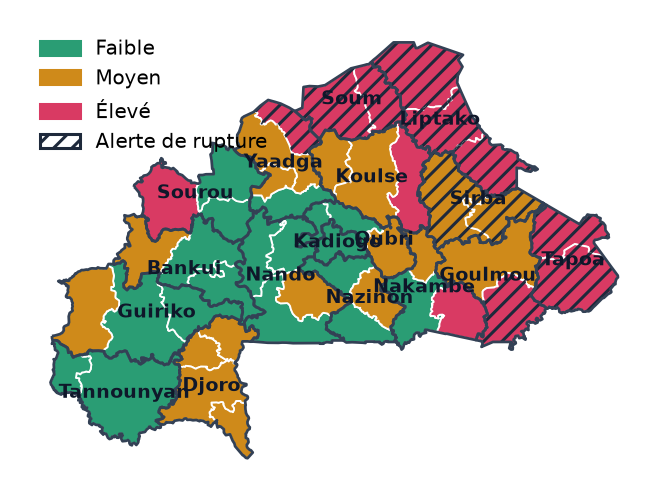
\includegraphics[width=\columnwidth]{fig_carte_2025_2026}
\caption{Classes de risque de décrochage prévues pour 2025-2026 (faible sous 8,4 \%, élevé au-delà de 14,2 \%) et provinces en alerte de rupture (hachures).}
\label{fig:carte}
\end{figure}

Pour 2025-2026, \textbf{12 provinces sont en risque élevé}, 17 en risque moyen et 18 en risque faible ; \textbf{11 sont en alerte de rupture} (figure~\ref{fig:carte}). Le risque se concentre dans le nord et l'est, là où la crise sécuritaire est la plus forte : les régions du Soum (23,2 \% en moyenne pondérée), du Liptako (21,4 \%) et de la Tapoa (15,8 \%) cumulent risque élevé et alertes de rupture. Le tableau~\ref{tab:top} donne les provinces les plus exposées.

\textbf{Taux et volume ne désignent pas les mêmes régions.} En nombre d'élèves, les régions les plus touchées sont les plus peuplées : le Yaadga (environ 42\,400 élèves en 2025-2026), le Guiriko (28\,000), le Koulsé (27\,200), le Nakambé (25\,500), le Nando (22\,100) et même le Kadiogo (20\,300), dont le taux n'est que de 3,3 \%. Le Soum, au taux le plus élevé, compte environ 2\,700 élèves concernés. L'outil donne les deux lectures : le taux pour l'urgence et l'intensité des actions, le volume pour dimensionner les moyens (tableau~\ref{tab:regions}).

\begin{table}[!htbp]
\centering
\footnotesize
\setlength{\tabcolsep}{4pt}
\begin{tabular}{@{}l r r r r r r@{}}
\toprule
& \multicolumn{3}{c}{Taux d'abandon (\%)} & Élèves & Risque & \\
Région & 24-25 & 25-26 & 27-28 & concernés & élevé & Alertes \\
\midrule
Soum & 18,7 & 23,2 & 24,4 & 2\,700 & 2 & 2 \\
Liptako & 18,5 & 21,4 & 22,1 & 10\,900 & 3 & 3 \\
Tapoa & 9,8 & 15,8 & 17,6 & 1\,900 & 2 & 2 \\
Yaadga & 10,2 & 12,0 & 12,6 & 42\,400 & 1 & 1 \\
Koulsé & 8,3 & 11,5 & 12,9 & 27\,200 & 1 & 0 \\
Sirba & 11,5 & 11,2 & 11,2 & 4\,200 & 0 & 2 \\
Djôrô & 8,5 & 10,3 & 10,8 & 14\,800 & 0 & 0 \\
Oubri & 10,8 & 9,6 & 9,3 & 19\,400 & 0 & 0 \\
Nakambé & 7,0 & 9,4 & 9,7 & 25\,500 & 1 & 0 \\
Sourou & 0,3 & 9,4 & 10,6 & 6\,700 & 1 & 0 \\
Goulmou & 8,0 & 9,1 & 9,4 & 7\,500 & 1 & 1 \\
Tannounyan & 6,1 & 7,9 & 8,4 & 10\,700 & 0 & 0 \\
Nazinon & 6,7 & 7,0 & 7,1 & 10\,800 & 0 & 0 \\
Guiriko & 7,0 & 6,7 & 7,0 & 28\,000 & 0 & 0 \\
Nando & 5,5 & 6,4 & 6,8 & 22\,100 & 0 & 0 \\
Bankui & 3,3 & 6,3 & 8,0 & 10\,900 & 0 & 0 \\
Kadiogo & 2,7 & 3,3 & 3,5 & 20\,300 & 0 & 0 \\
\midrule
Burkina Faso & 6,7 & 8,0 & 8,5 & 266\,100 & 12 & 11 \\
\bottomrule
\end{tabular}
\caption{Les 17 régions : taux pondéré par les effectifs (observé en 2024-2025, prévu ensuite), nombre estimé d'élèves qui abandonnent en 2025-2026, provinces en risque élevé et en alerte de rupture. Le taux observé du Sourou en 2024-2025 est tiré vers le bas par une valeur publiée négative (Kossin).}
\label{tab:regions}
\end{table}

\begin{table}[!htbp]
\centering
\footnotesize
\setlength{\tabcolsep}{3.5pt}
\begin{tabular}{@{}l l r r r c@{}}
\toprule
Province & Région & 24-25 & 25-26 [IC 80 \%] & 27-28 & Rupture \\
\midrule
Loroum & Yaadga & 34,4 & 27,1 [13,1 ; 47,8] & 25,5 & élevée \\
Karo-Peli & Soum & 18,7 & 23,6 [11,1 ; 43,1] & 24,8 & élevée \\
Djelgodji & Soum & 18,7 & 23,2 [10,9 ; 42,6] & 24,3 & élevée \\
Séno & Liptako & 18,3 & 23,0 [10,8 ; 42,4] & 24,2 & élevée \\
Yagha & Liptako & 19,4 & 22,8 [10,7 ; 42,1] & 23,6 & élevée \\
Oudalan & Liptako & 18,7 & 18,6 [8,5 ; 36,0] & 18,6 & élevée \\
Kossin & Sourou & $-$1,4 & 16,2 [7,3 ; 32,4] & 16,2 & faible \\
Namentenga & Koulsé & 17,2 & 15,9 [7,1 ; 31,8] & 15,6 & moyenne \\
Gobnangou & Tapoa & 9,7 & 15,8 [7,1 ; 31,6] & 17,6 & élevée \\
Dyamongou & Tapoa & 9,7 & 15,8 [7,1 ; 31,6] & 17,6 & élevée \\
Kompienga & Goulmou & 13,4 & 14,7 [6,5 ; 29,9] & 15,1 & élevée \\
Koulpélogo & Nakambé & 3,3 & 14,4 [6,4 ; 29,3] & 14,4 & faible \\
\bottomrule
\end{tabular}
\caption{Les 12 provinces en risque élevé en 2025-2026 : taux d'abandon (\%) observé, prévu avec son intervalle à 80 \%, projeté en 2027-2028, et classe de rupture. Une valeur publiée négative (Kossin, Koulpélogo bas) est ramenée vers le niveau habituel par le modèle.}
\label{tab:top}
\end{table}

\subsection{Comment le risque va évoluer}

\begin{figure}[!htbp]
\centering
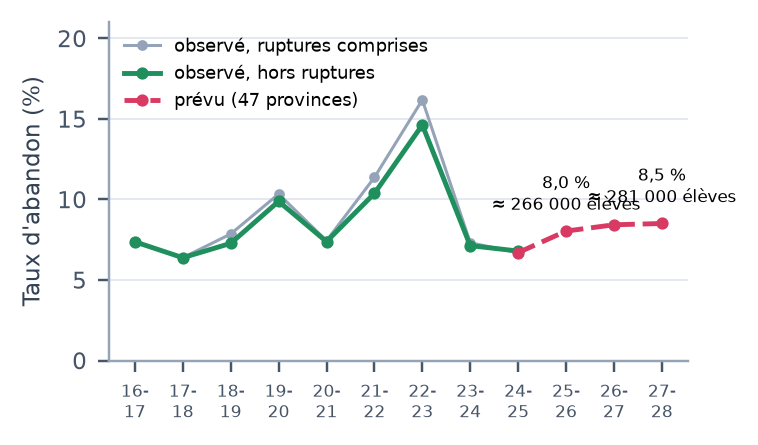
\includegraphics[width=\columnwidth]{fig_trajectoire_nationale}
\caption{Taux d'abandon national (moyenne des provinces pondérée par les effectifs) : observé de 2016-2017 à 2024-2025, prévu jusqu'en 2027-2028, avec le nombre estimé d'élèves qui abandonnent.}
\label{fig:national}
\end{figure}

\begin{figure*}[!t]
\centering
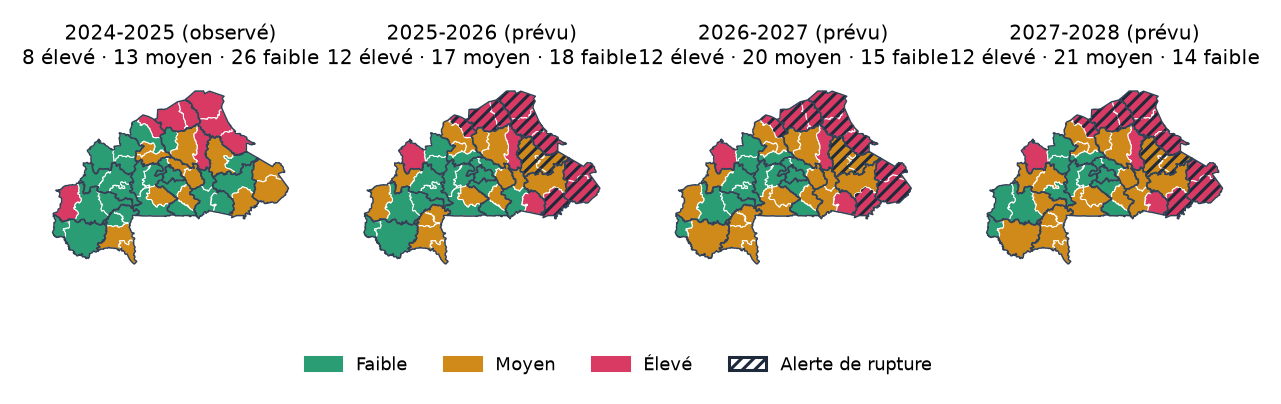
\includegraphics[width=\textwidth]{fig_cartes_annees}
\caption{Classes de risque de l'année observée aux trois années prévues : le cœur du risque reste au nord et à l'est, et la classe moyenne s'étend vers le centre au fil des années.}
\label{fig:cartes_annees}
\end{figure*}

\textbf{Le taux national remonte.} Après le pic de 2022-2023, l'année 2024-2025 a été exceptionnellement basse (6,7 \%). Le modèle prévoit \textbf{8,0 \% en 2025-2026}, puis 8,4 et 8,5 \% : environ \textbf{266\,000 élèves} en 2025-2026 et 282\,000 en 2027-2028, si les effectifs restent ceux de 2024-2025 (figure~\ref{fig:national}). Cette remontée n'est pas une tendance inventée : de nombreuses provinces étaient en 2024-2025 sous leur niveau habituel, et le retour amorti les y ramène progressivement.

\begin{figure}[!htbp]
\centering
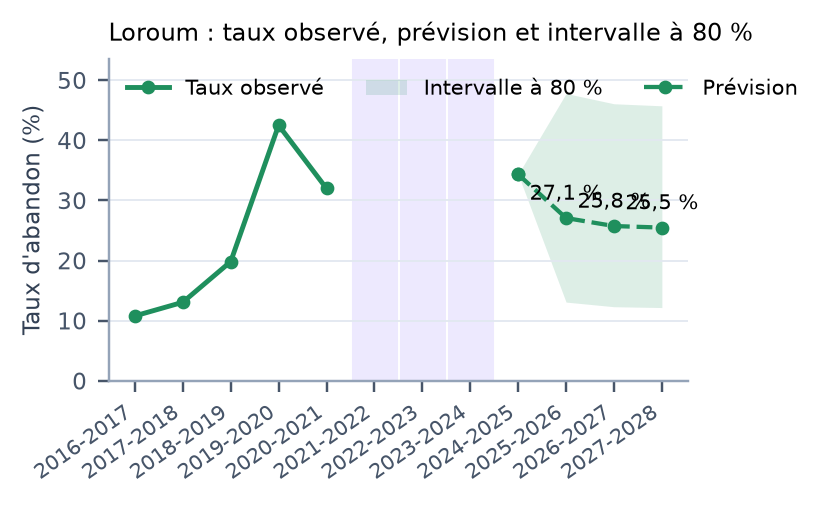
\includegraphics[width=\columnwidth]{fig_trajectoire_loroum}
\caption{Loroum : taux observés, années de rupture (bandes), prévision et intervalle à 80 \%. Le taux exceptionnel de 2024-2025 revient vers le niveau habituel de la province.}
\label{fig:loroum}
\end{figure}

\textbf{Province par province, la logique est lisible.} Le Loroum, au taux exceptionnel de 34,4 \% en 2024-2025, redescend vers son niveau habituel : 27,1 \%, puis 25,8 et 25,5 \% (figure~\ref{fig:loroum}). À l'inverse, les provinces du Soum et du Liptako, qui ont connu une accalmie en 2024-2025, remontent vers 23 à 25 \%. Le nombre de provinces en risque moyen passe de 17 à 21 entre 2025-2026 et 2027-2028 (figures~\ref{fig:classes} et~\ref{fig:cartes_annees}) ; dans le tableau de bord, le curseur des années fait défiler ces changements sur la carte (figure~\ref{fig:ecran2028}).

\begin{figure*}[!t]
\centering
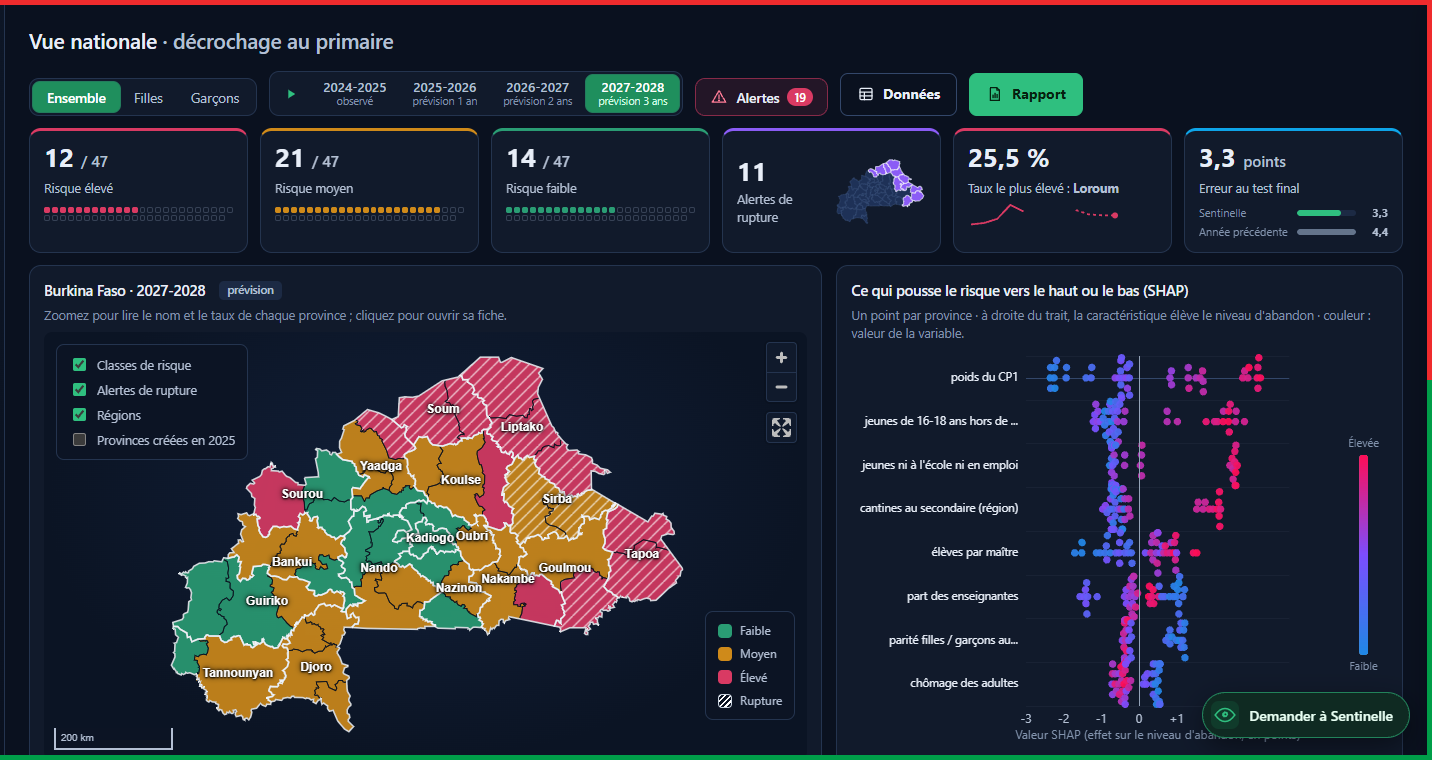
\includegraphics[width=0.86\textwidth]{ecran_nationale_2028}
\caption{La vue nationale positionnée sur 2027-2028 : 12 provinces en risque élevé, 21 en risque moyen ; l'erreur au test et le taux le plus élevé restent affichés en tête.}
\label{fig:ecran2028}
\end{figure*}

\begin{figure}[!htbp]
\centering
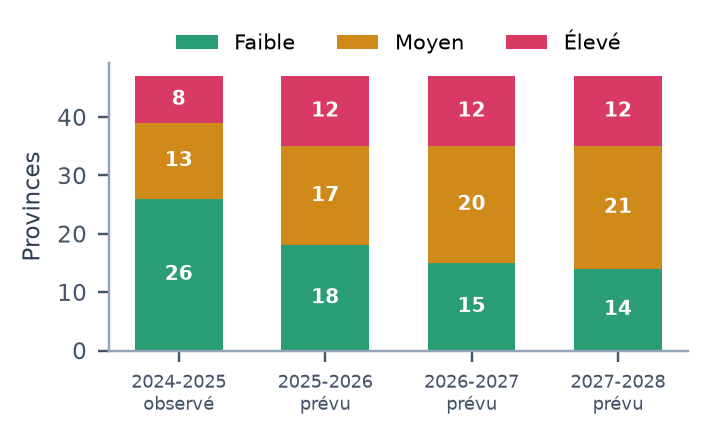
\includegraphics[width=\columnwidth]{fig_classes_par_annee}
\caption{Provinces par classe de risque, de l'année observée aux trois années prévues.}
\label{fig:classes}
\end{figure}

\subsection{Pourquoi : les facteurs du risque}

\begin{figure}[!htbp]
\centering
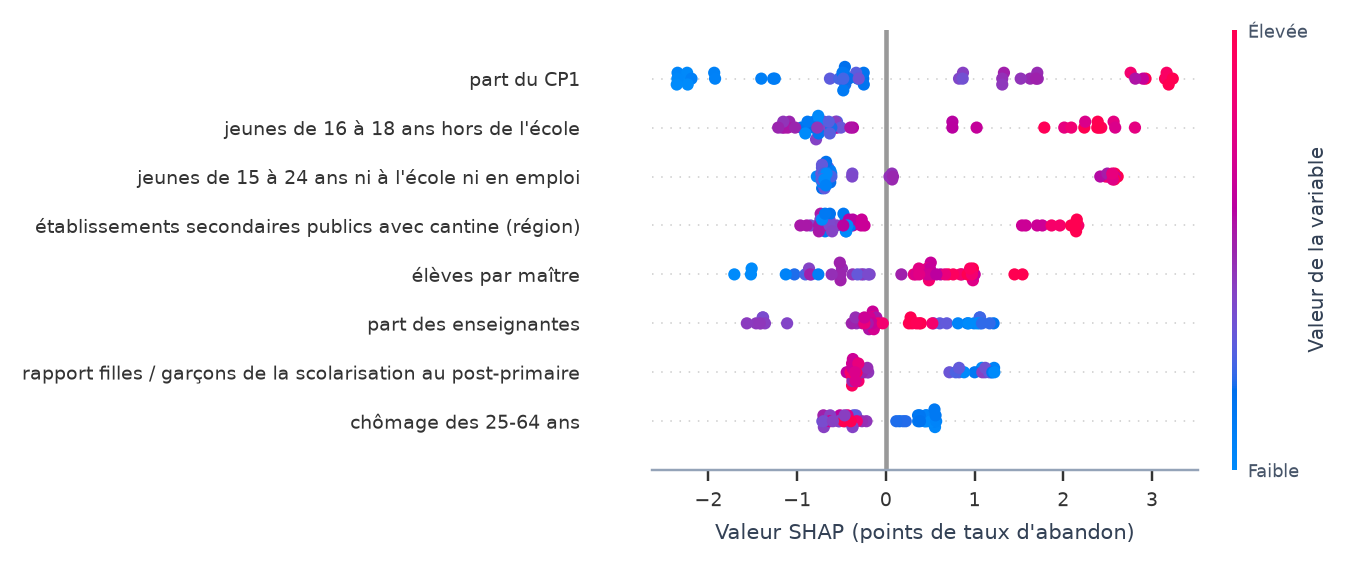
\includegraphics[width=\columnwidth]{fig_shap}
\caption{Valeurs SHAP : un point par province ; à droite du trait, la variable élève le niveau habituel d'abandon ; la couleur donne la valeur de la variable.}
\label{fig:shap}
\end{figure}

\begin{table}[!t]
\centering
\footnotesize
\begin{tabularx}{\columnwidth}{@{}Y r@{}}
\toprule
Variable (elastic net, provinces non vues : $R^2 = 0{,}64$) & Effet sur le niveau habituel \\
\midrule
Poids du CP1 dans les effectifs & +0,97 point par point de \% \\
Jeunes de 15-24 ans ni à l'école ni en emploi & +0,08 point par point de \% \\
Places assises manquantes pour 100 élèves & +0,16 point par place \\
\bottomrule
\end{tabularx}
\caption{Effets chiffrés utilisés par le simulateur de leviers (associations mesurées entre provinces, toutes choses égales par ailleurs dans le modèle).}
\label{tab:effets}
\end{table}

La figure~\ref{fig:shap} montre, province par province, ce qui élève ou abaisse le niveau habituel d'abandon. \textbf{Le poids du CP1} vient en tête : une province où le CP1 pèse lourd dans les effectifs perd ses élèves au fil du cycle (jusqu'à +3,2 points). Viennent ensuite \textbf{les jeunes de 16 à 18 ans hors de l'école}, \textbf{les jeunes ni à l'école ni en emploi} (l'école perd son sens quand elle ne débouche sur rien) et \textbf{le nombre d'élèves par maître}. Une part plus élevée d'enseignantes va de pair avec un risque plus faible. Le tableau~\ref{tab:effets} chiffre les effets retenus par l'elastic net : un point de pourcentage de plus pour le poids du CP1 s'accompagne d'un niveau d'abandon plus élevé de près d'un point.

\begin{figure}[!htbp]
\centering
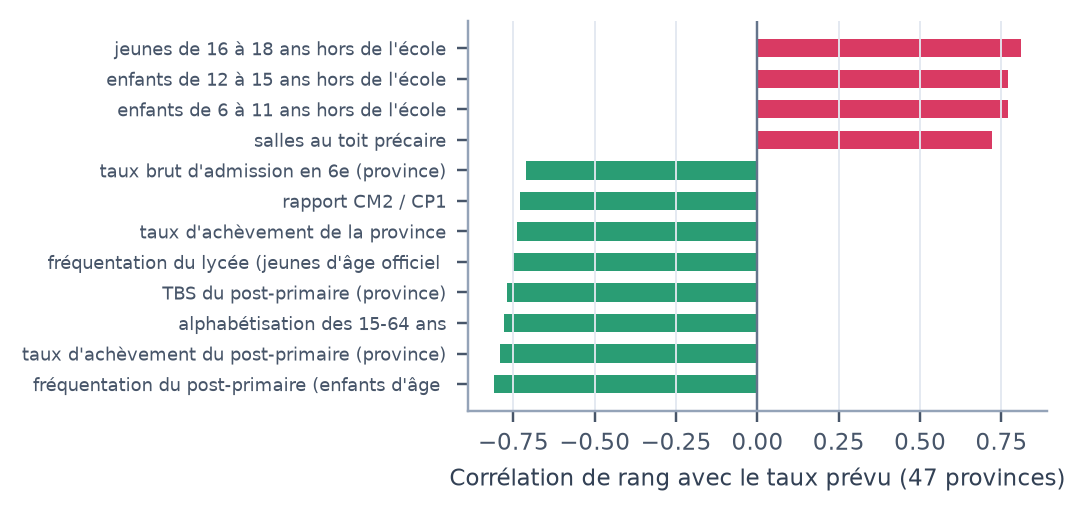
\includegraphics[width=\columnwidth]{fig_liens_indicateurs}
\caption{Indicateurs les plus liés au taux prévu (corrélation de rang sur les 47 provinces) : rouge, plus l'indicateur est élevé, plus le risque l'est ; vert, l'inverse.}
\label{fig:liens}
\end{figure}

Au-delà des variables du modèle, les 64 indicateurs de la base sont reliés au risque (figure~\ref{fig:liens}). Les provinces où \textbf{les enfants sont hors de l'école} (corrélation de 0,77 à 0,81), où \textbf{les filles sont mariées tôt} (0,70) et où les salles sont précaires ont un taux prévu plus élevé ; celles où le post-primaire est fréquenté et achevé, où les adultes sont alphabétisés (de $-0{,}74$ à $-0{,}81$) et où les écoles sont électrifiées ($-0{,}51$) en ont un plus faible. Ce sont des associations entre provinces, pas des causes démontrées : elles orientent l'analyse, elles ne prouvent pas l'effet d'une mesure.

\subsection{Ce qui va mieux qu'attendu, et pour qui}

\begin{figure}[!htbp]
\centering
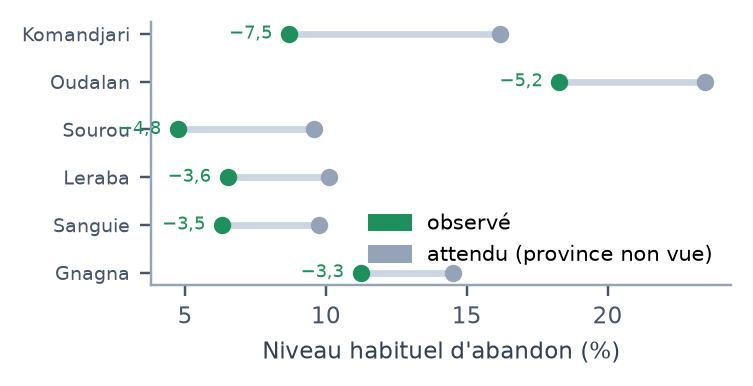
\includegraphics[width=\columnwidth]{fig_resistantes}
\caption{Provinces qui résistent : niveau habituel observé, nettement sous celui attendu d'après leurs caractéristiques (prédit sans voir la province).}
\label{fig:resistantes}
\end{figure}

\textbf{Des provinces résistent.} Le Komandjari a un niveau habituel de 8,7 \% alors que ses caractéristiques en laissaient attendre 16,2 \% ; l'Oudalan, le Sourou, la Léraba et le Sanguié font aussi mieux que prévu (figure~\ref{fig:resistantes}). L'écart est mesuré avec un modèle qui n'a pas vu la province : ce n'est pas un artefact d'ajustement. Ces provinces sont des terrains à étudier, et si leurs pratiques se confirment, à reproduire.

\begin{figure}[!htbp]
\centering
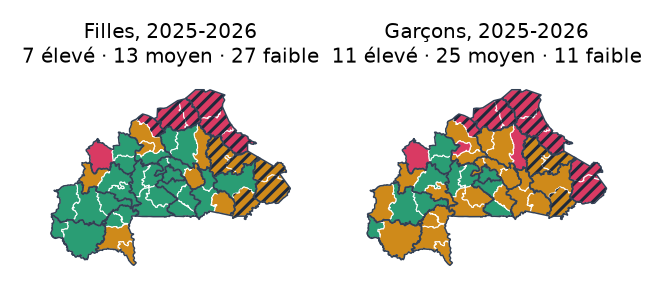
\includegraphics[width=\columnwidth]{fig_cartes_sexe}
\caption{Classes de risque prévues pour 2025-2026, filles et garçons (seuils propres au modèle par sexe).}
\label{fig:cartes_sexe}
\end{figure}

\textbf{Les garçons décrochent davantage} au primaire (figure~\ref{fig:cartes_sexe}) : leur taux prévu dépasse celui des filles dans 39 provinces sur 47 (12,1 \% contre 9,5 \% en moyenne). Les filles sont plus exposées dans le Liptako : dans le Séno (+3,1 points) et le Yagha (+1,8 point), où le mariage précoce est très fréquent (65 \% des filles de 17 ans sont mariées dans le Yagha, contre 32 \% en médiane) (figure~\ref{fig:fg}).

\begin{figure}[!htbp]
\centering
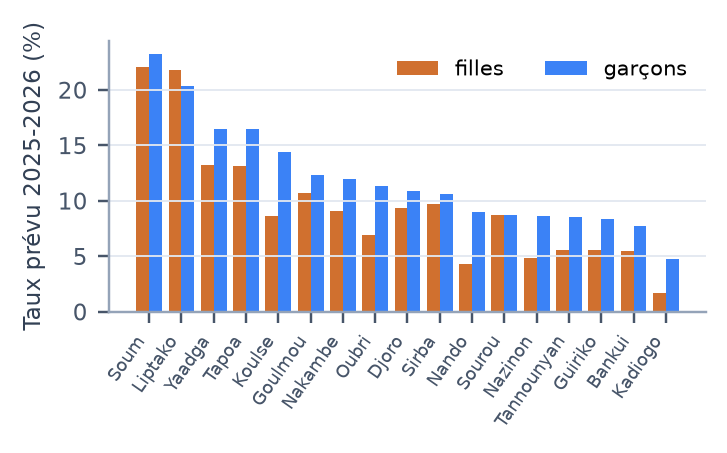
\includegraphics[width=\columnwidth]{fig_filles_garcons}
\caption{Taux d'abandon prévu en 2025-2026, filles et garçons, par région (moyenne des provinces).}
\label{fig:fg}
\end{figure}

%======================================================================
\section{La réponse au défi : l'application \sol{}}
%======================================================================

\sol{} n'est pas un rapport figé : c'est un outil en service, en ligne (\lien), qui fonctionne aussi sans Internet sur un simple ordinateur. Il s'adresse à un décideur sans compétence technique et répond à quatre questions : \emph{où agir}, \emph{pourquoi}, \emph{avec quels leviers}, et \emph{comment suivre la situation d'une année à l'autre}.

\subsection{Architecture et choix techniques}

\begin{figure}[!htbp]
\centering
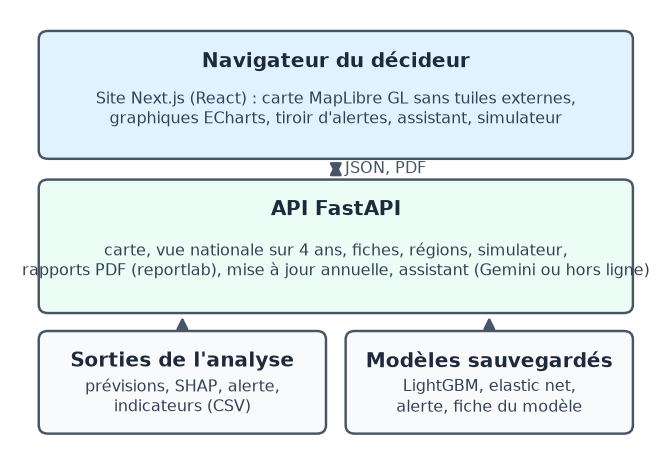
\includegraphics[width=\columnwidth]{fig_architecture}
\caption{Architecture : un site web lit une API qui sert les sorties de l'analyse et les modèles sauvegardés, sans jamais recalculer en cachette.}
\label{fig:architecture}
\end{figure}

L'application sépare deux parties (figure~\ref{fig:architecture}). Une \textbf{API FastAPI} sert les sorties de l'analyse et les modèles sauvegardés : elle ne recalcule aucune prévision, si bien que les chiffres affichés sont exactement ceux de l'analyse et des dépôts. Un \textbf{site Next.js} (React) affiche la carte avec MapLibre GL, sans aucune tuile externe (les contours viennent de nos données), et les graphiques avec ECharts. L'ensemble tient dans une seule image Docker. Il est déployé en ligne sur un hébergeur de conteneurs, et se lance hors ligne par un double clic (\texttt{lancer.bat}). Les couleurs des classes de risque et des filles et garçons ont été choisies et vérifiées pour être distinguées par les personnes daltoniennes. Chaque écran tient sur une hauteur d'écran, avec peu de texte : l'information se lit sur la carte et les graphiques, et le détail apparaît au survol.

\subsection{La vue nationale : où agir}

La vue nationale (figure~\ref{fig:ecran}) réunit sur un écran : six chiffres clés (provinces par classe de risque avec une bande des 47 provinces, alertes de rupture avec leur mini-carte, taux le plus élevé, erreur au test comparée à la méthode naïve) ; la carte, où l'on zoome pour lire le nom et le taux de chaque province ; le nuage SHAP ; le classement des 47 provinces en trois graphiques ; les filles et les garçons par région ; les provinces qui résistent ; et l'évolution des classes d'une année à l'autre. Une bascule affiche l'ensemble des élèves, les filles ou les garçons ; un curseur choisit l'année, de 2024-2025 observé à 2027-2028, et un bouton de lecture fait défiler les années.

\begin{figure*}[!t]
\centering
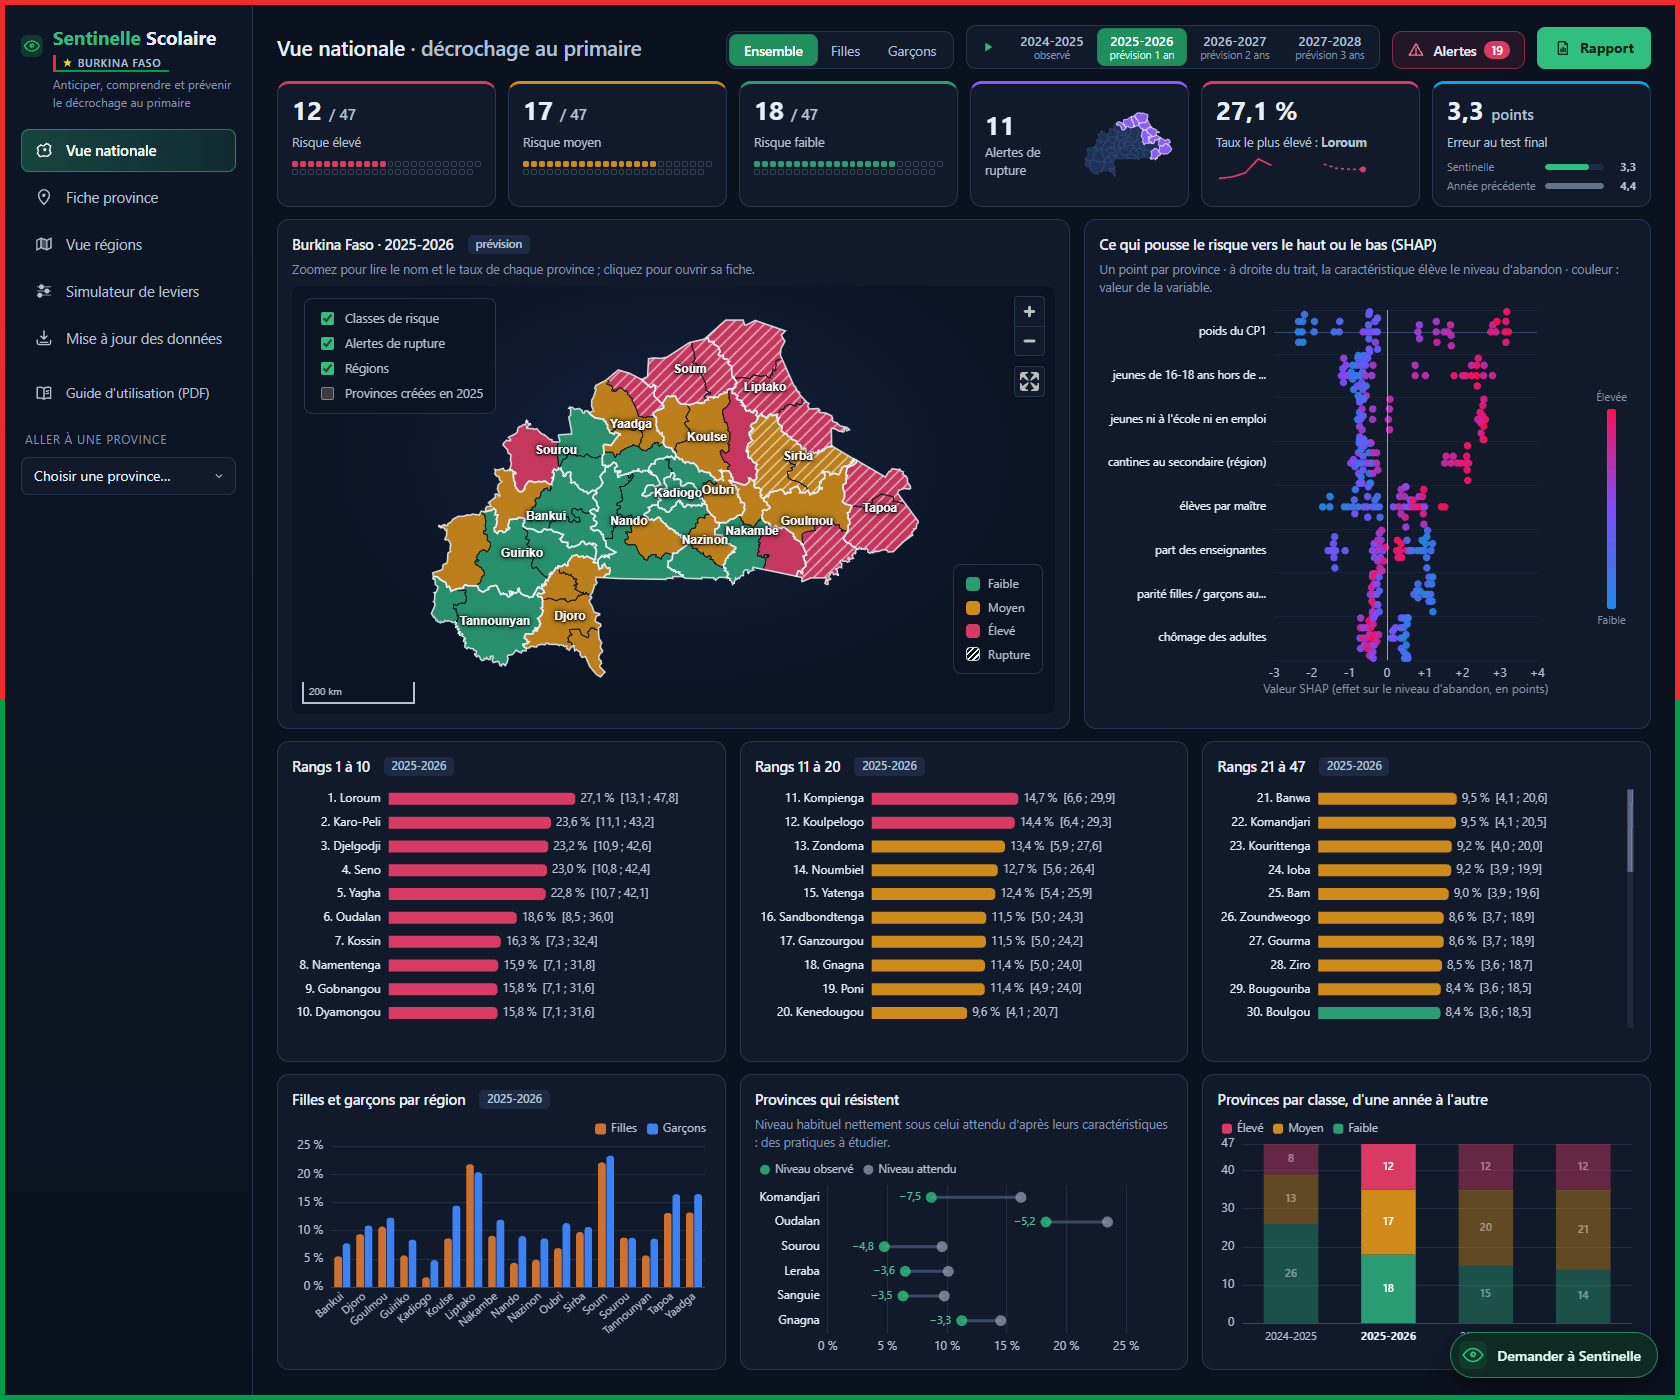
\includegraphics[width=\textwidth]{ecran_nationale}
\caption{Vue nationale du tableau de bord en ligne (prévision 2025-2026).}
\label{fig:ecran}
\end{figure*}

\textbf{Les alertes} sont rangées dans un panneau latéral, ouvert par un bouton à compteur : provinces en alerte de rupture avec leur score, et provinces en risque élevé dont le taux prévu dépasse celui de l'année (figure~\ref{fig:majal}). Un clic ouvre la fiche de la province.

\subsection{La fiche province : comprendre un territoire}

La fiche d'une province tient sur un écran (figure~\ref{fig:ecrans}) : taux observé en 2024-2025, prévision 2025-2026 avec sa variation et son intervalle, classe et rang, score de rupture, niveau attendu d'après ses caractéristiques, petite carte de situation ; puis l'historique depuis 2016-2017 avec les années de rupture et les prévisions jusqu'en 2027-2028, la cascade SHAP de ses facteurs, les taux des filles et des garçons et la jauge de rupture. La même fiche se lit pour les filles ou pour les garçons. Un bouton produit la fiche de décision en PDF.

\begin{figure*}[!t]
\centering
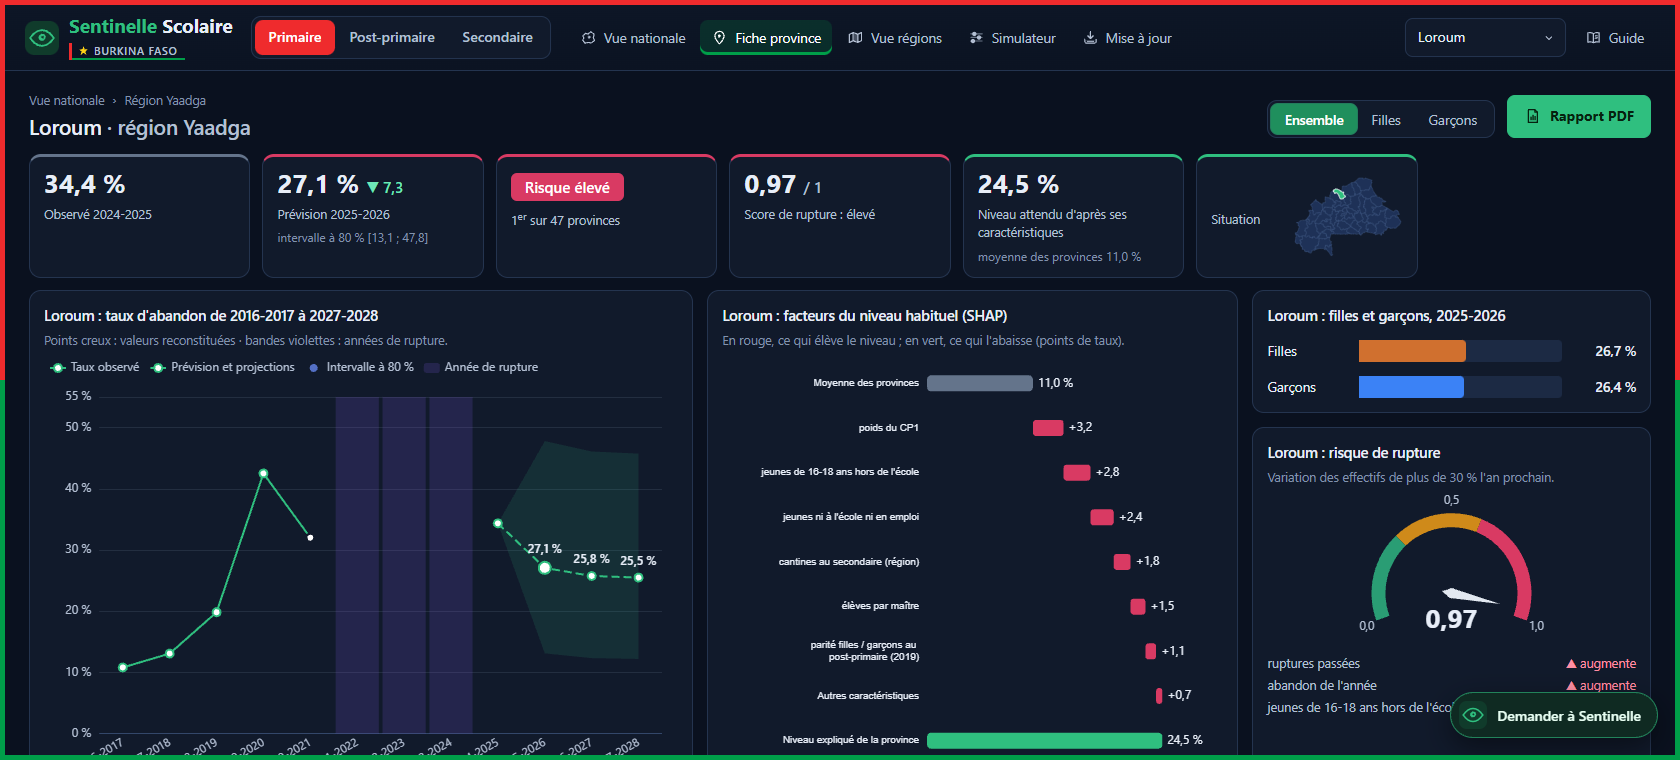
\includegraphics[height=5.4cm]{ecran_province}\hfill
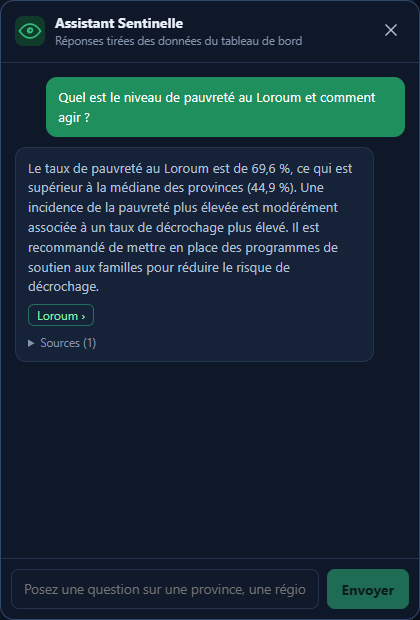
\includegraphics[height=5.4cm]{ecran_assistant}
\caption{À gauche, fiche d'une province (Loroum). À droite, l'assistant répond à partir des données et cite ses sources.}
\label{fig:ecrans}
\end{figure*}

\begin{figure*}[!t]
\centering
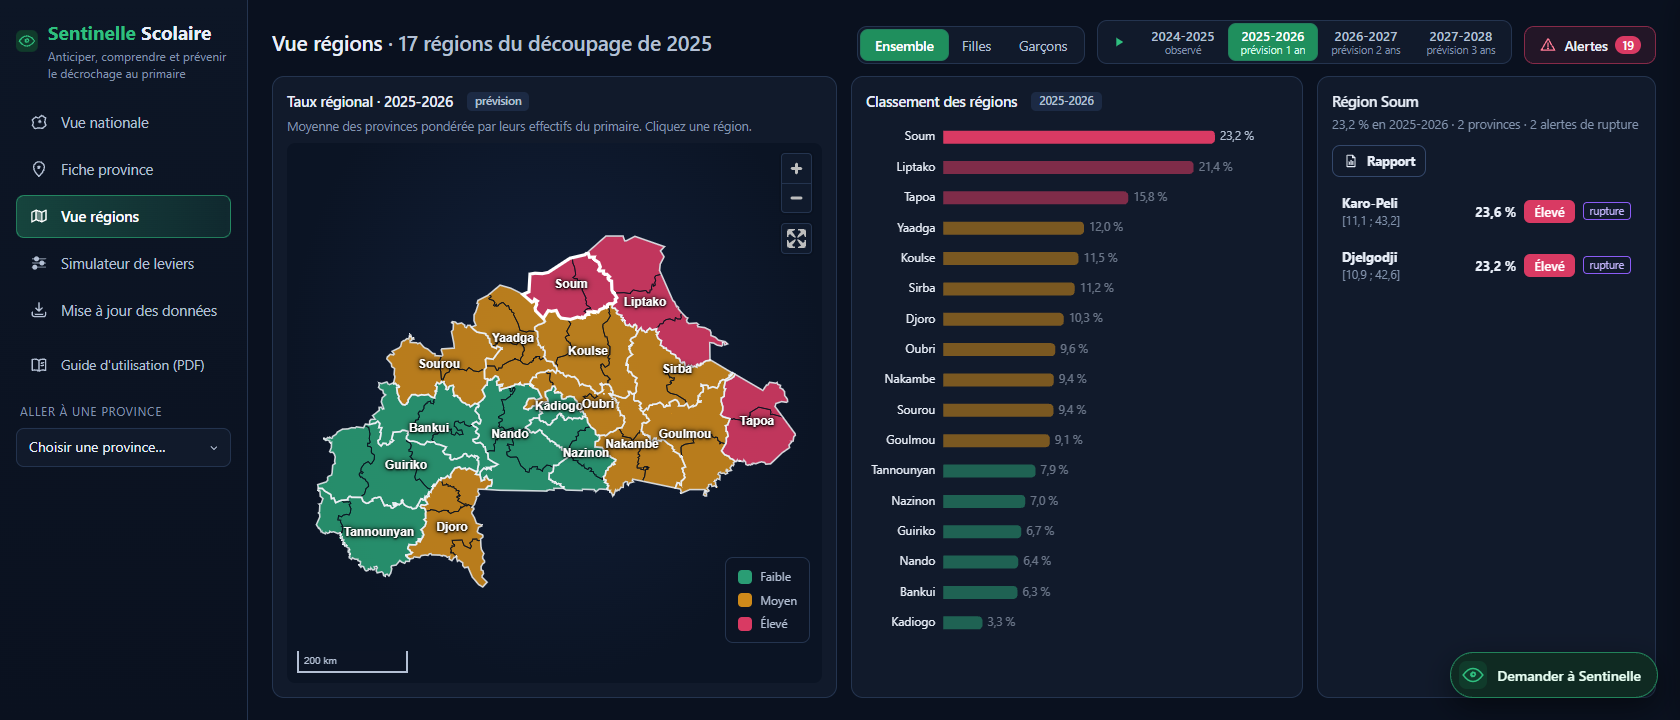
\includegraphics[width=0.495\textwidth]{ecran_regions}\hfill
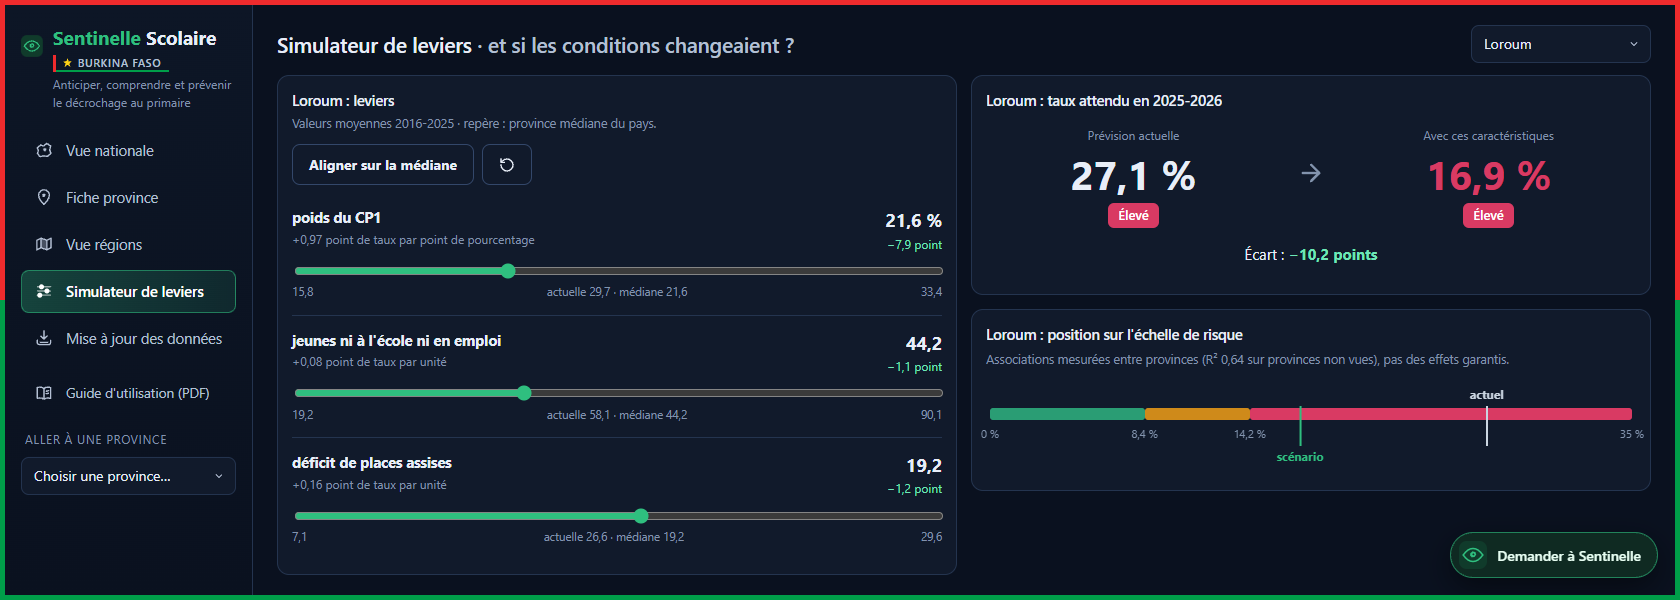
\includegraphics[width=0.495\textwidth]{ecran_simulateur}
\caption{À gauche, la vue régions : carte, classement des 17 régions et provinces de la région choisie (Soum). À droite, le simulateur de leviers : le Loroum aligné sur la province médiane.}
\label{fig:regsim}
\end{figure*}

\subsection{La vue régions : piloter un territoire}

La vue régions (figure~\ref{fig:regsim}) colore les 17 régions selon leur taux pondéré par les effectifs, les classe, et liste les provinces de la région choisie avec leur intervalle, leur classe et leur alerte. Elle suit le même curseur des années et produit le rapport régional en PDF.

\subsection{Le simulateur : avec quels leviers}

Le simulateur (figure~\ref{fig:regsim}) répond à « et si les conditions changeaient ? ». Pour une province, on déplace trois curseurs, le poids du CP1, les jeunes ni à l'école ni en emploi et les places assises manquantes, et l'outil recalcule le niveau attendu avec l'elastic net sauvegardé. Aligner le Loroum sur la province médiane du pays abaisserait son niveau attendu d'environ 10 points, de 27,1 \% à 17 \% environ. C'est un ordre de grandeur pour hiérarchiser les priorités, pas un effet garanti : le simulateur l'écrit en clair.

\subsection{Les rapports PDF : décider hors de l'écran}

Chaque vue produit un rapport à imprimer ou à transmettre, généré à la demande avec les mêmes chiffres que l'écran (figure~\ref{fig:rapports}) : un \textbf{rapport national} (chiffres clés, carte, quinze provinces les plus exposées, provinces qui résistent, facteurs, pistes d'action), un \textbf{rapport par région} et une \textbf{fiche par province} (prévision, évolution, cascade des facteurs, filles et garçons, rupture, pistes d'action liées à ses facteurs). Les 47 fiches et les 17 rapports régionaux sont aussi déposés avec l'étape 05.

\begin{figure*}[!t]
\centering
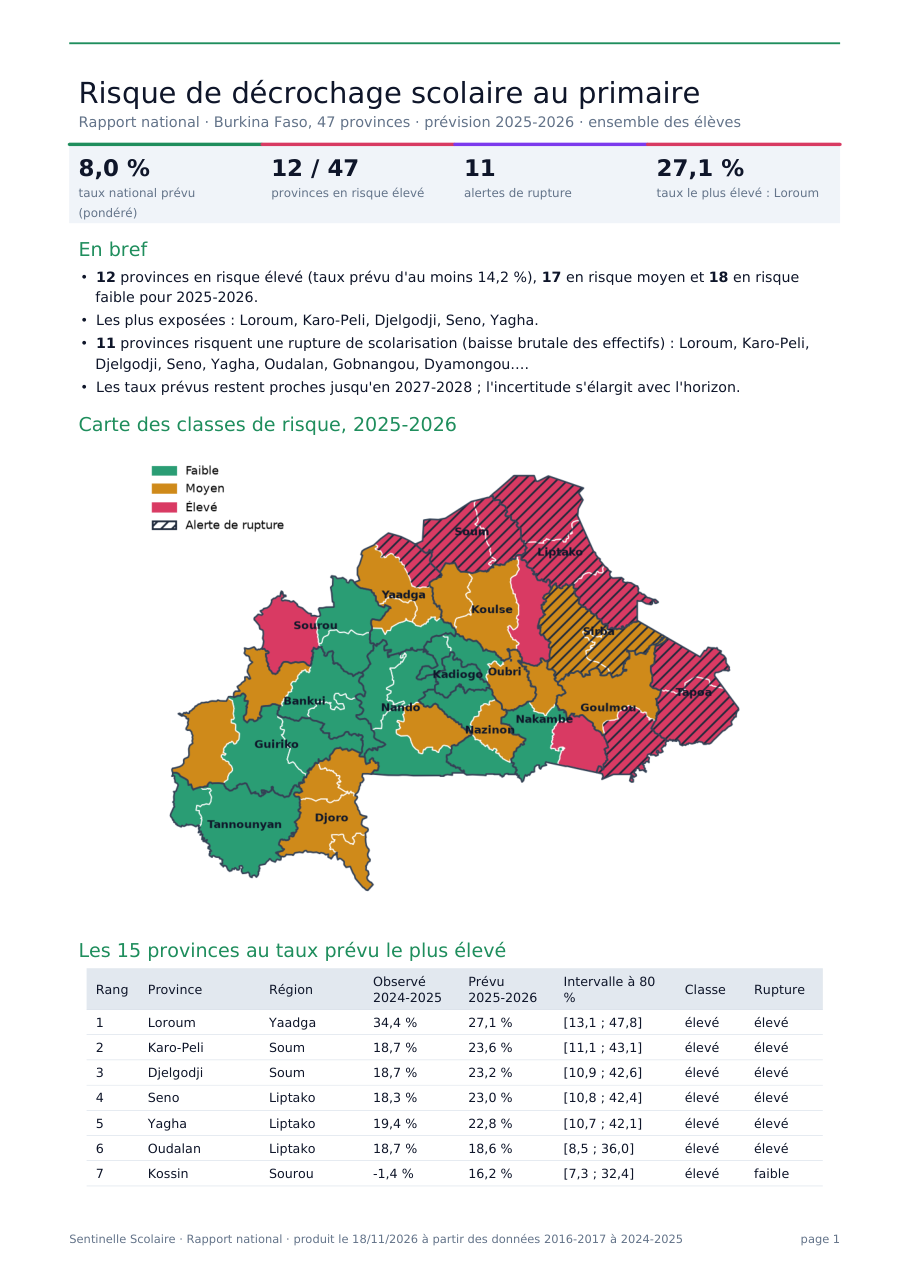
\includegraphics[width=0.32\textwidth]{rapport_national_p1}\hfill
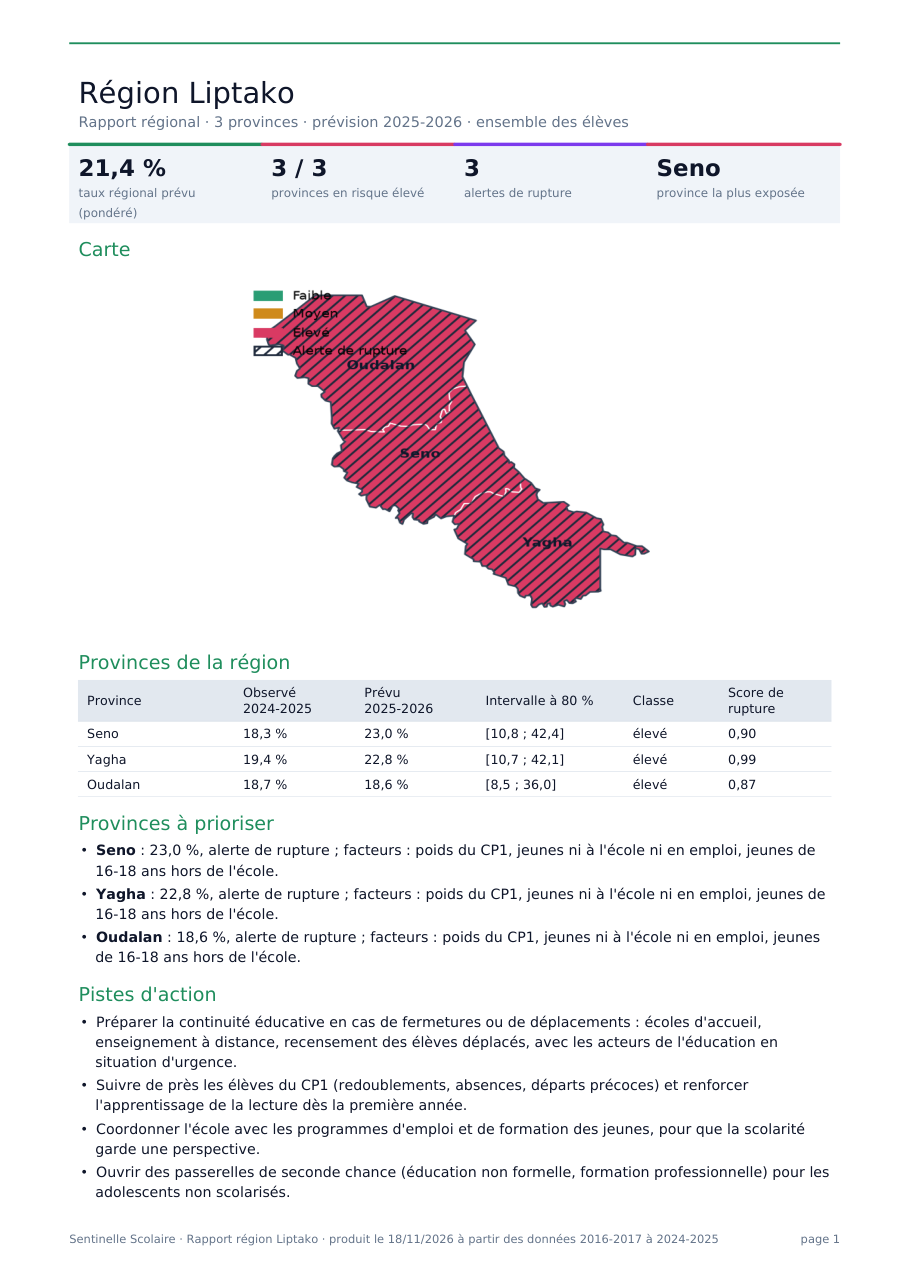
\includegraphics[width=0.32\textwidth]{rapport_region_liptako}\hfill
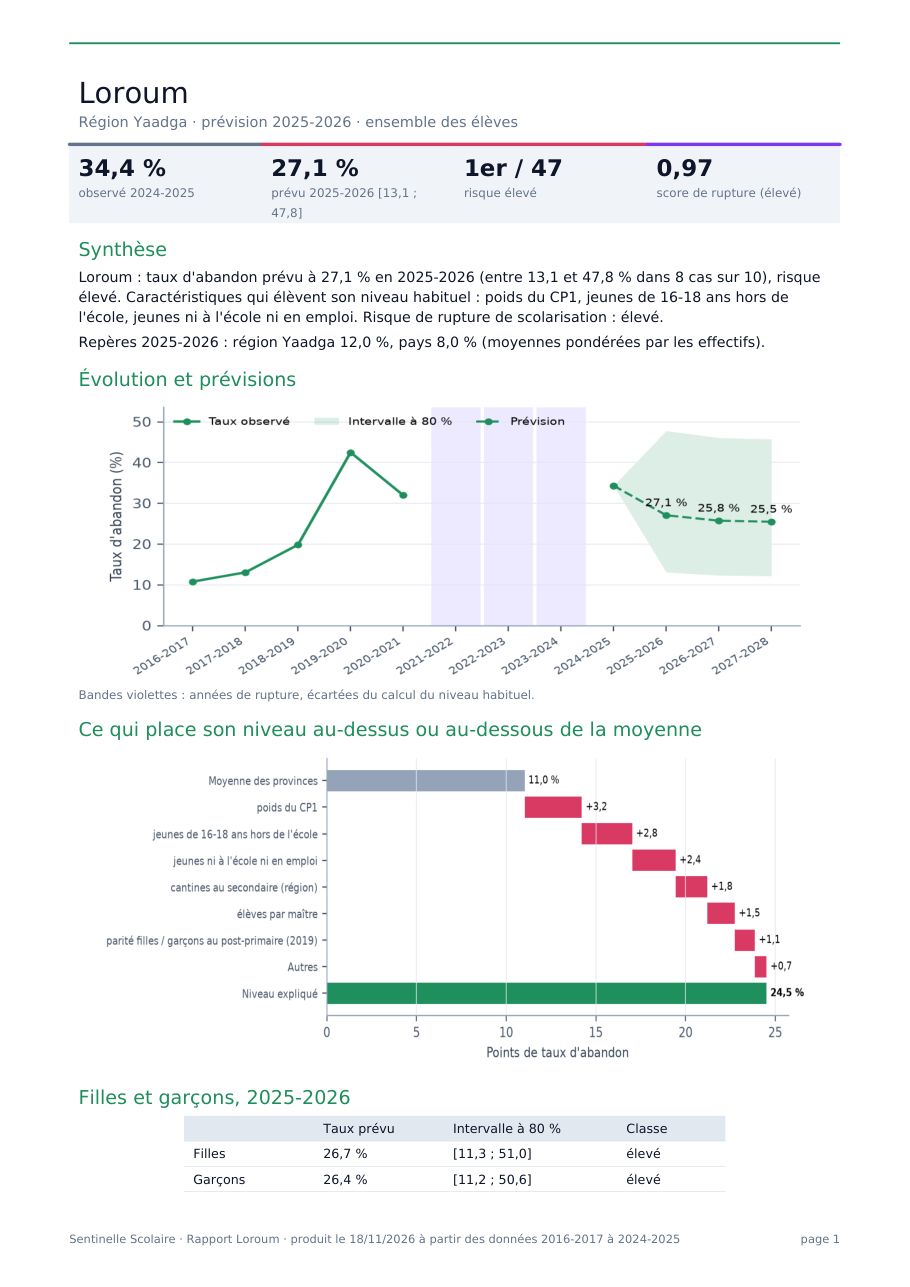
\includegraphics[width=0.32\textwidth]{rapport_fiche_loroum}
\caption{Rapports générés automatiquement : rapport national, rapport de la région du Liptako, fiche de la province du Loroum (premières pages).}
\label{fig:rapports}
\end{figure*}

\subsection{L'assistant : poser sa question}

L'assistant, ouvert depuis n'importe quel écran, répond en français aux questions d'un décideur : « où agir en priorité ? », « compare le Loroum et le Yagha », « quel est le niveau de pauvreté au Loroum ? », « où les cantines manquent-elles le plus ? ». Il interroge les données du tableau de bord par des fonctions dédiées (fiche d'une province, classements, synthèse d'une région, alertes, provinces qui résistent, et les 64 indicateurs de la base avec leur médiane, leur rang et leur lien avec le risque) ; il tient compte de l'échange précédent (« la zone » désigne la région dont on vient de parler) et cite ses sources. Les chiffres viennent toujours de ces fonctions, jamais d'une invention ; sans connexion, un mode hors ligne répond aux mêmes questions. Seules des statistiques agrégées par province sont transmises, aucune donnée individuelle.

\begin{figure*}[!t]
\centering
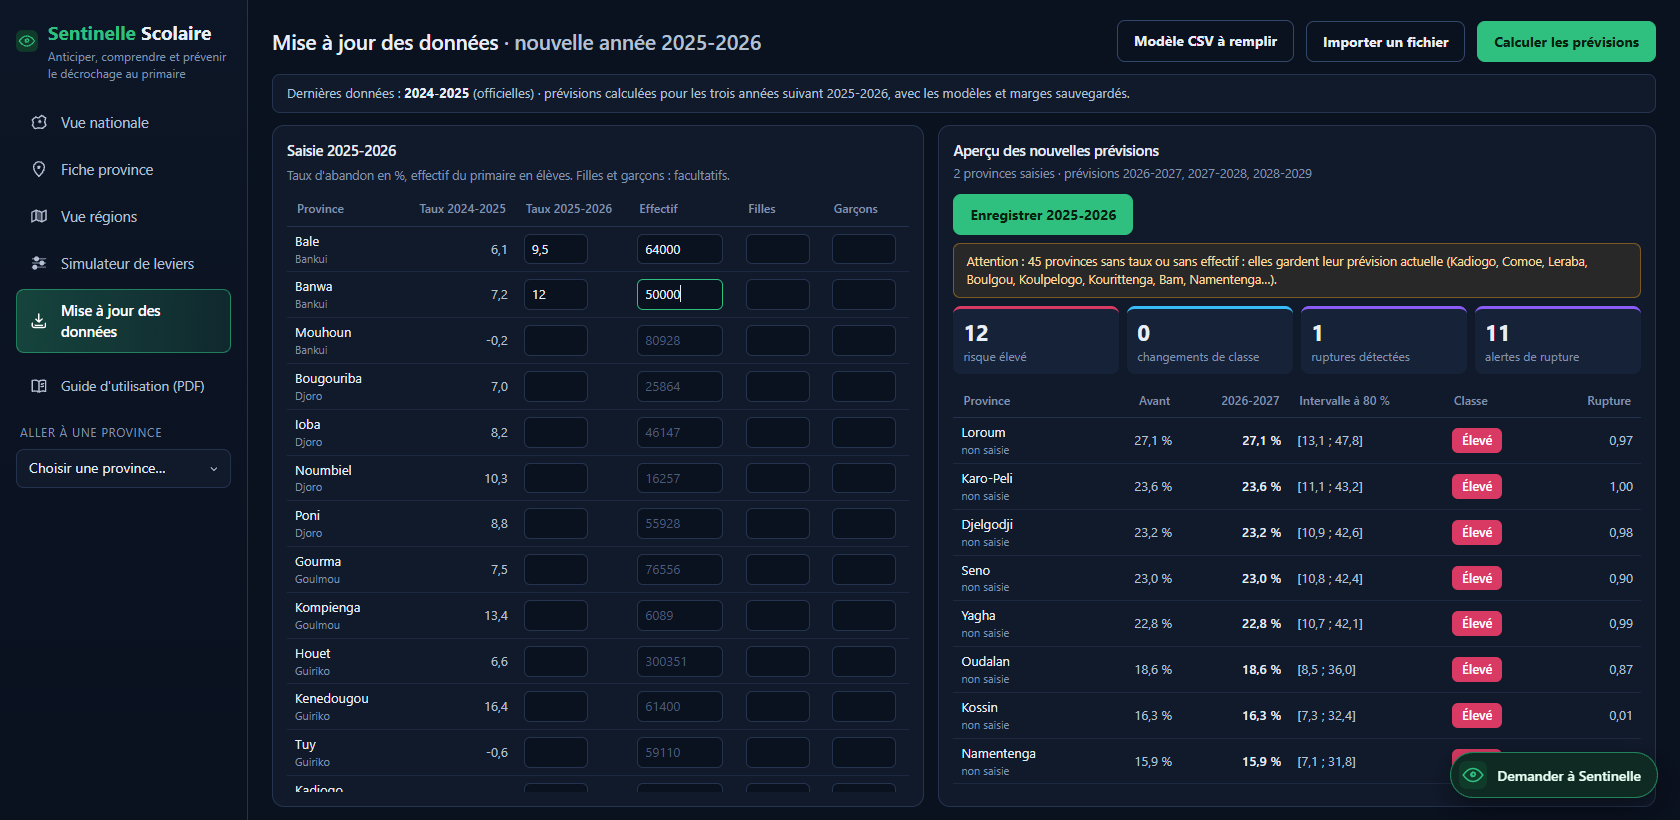
\includegraphics[height=5.1cm]{ecran_mise_a_jour}\hfill
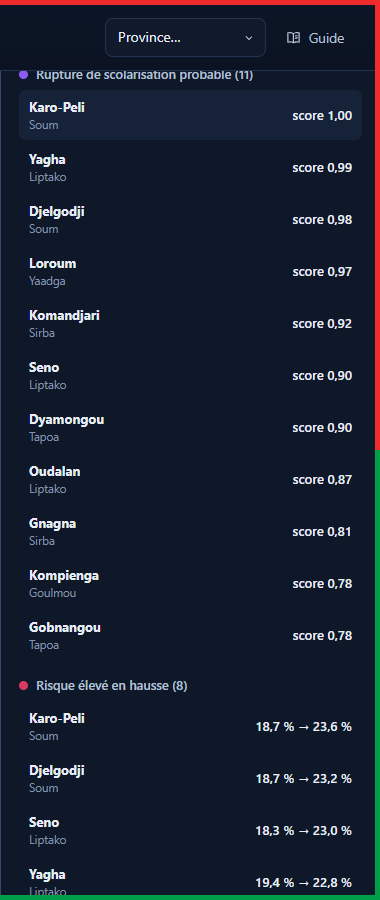
\includegraphics[height=5.1cm]{ecran_alertes}
\caption{À gauche, la mise à jour annuelle : saisie, contrôles, nouvelles prévisions et changements de classe. À droite, le panneau des alertes : ruptures probables et risques élevés en hausse.}
\label{fig:majal}
\end{figure*}

\subsection{La mise à jour annuelle : un outil qui dure}

Un outil de prévision ne vaut que s'il se tient à jour. À la sortie de l'annuaire, le service statistique télécharge un fichier modèle (47 provinces, valeurs de l'année précédente pour repère), y reporte le taux d'abandon et l'effectif de chaque province, ou les saisit à l'écran, puis lance le calcul (figure~\ref{fig:majal}). L'outil contrôle les données (provinces manquantes, valeurs impossibles, ruptures détectées), recalcule les prévisions des trois années suivantes et le score de rupture avec les modèles sauvegardés, et montre les changements de classe avant tout enregistrement. Le calcul reproduit exactement celui de l'analyse (écart nul sur les 47 provinces), et les données saisies sont rangées à part des données officielles, que l'on retrouve d'un clic.

\begin{figure*}[!t]
\centering
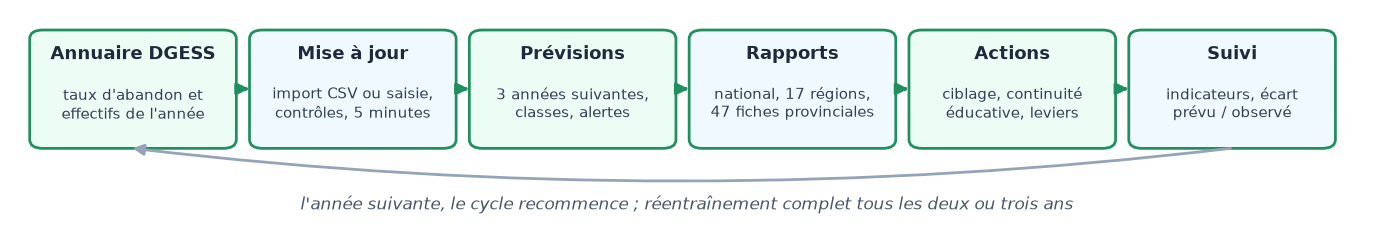
\includegraphics[width=0.96\textwidth]{fig_cycle_annuel}
\caption{Cycle annuel d'utilisation de \sol{} par l'administration.}
\label{fig:cycle}
\end{figure*}

\subsection{Un parcours de décision}

Une directrice régionale du Liptako prépare sa rentrée. Sur la vue nationale, la carte lui montre trois provinces de sa région en rouge et hachurées. La fiche du Séno donne 23 \% prévus, entre 11 et 42 \% dans huit cas sur dix, une alerte de rupture élevée, et des facteurs : jeunes hors de l'école, poids du CP1. En vue filles, le taux est plus élevé encore, et l'assistant lui apprend que le mariage précoce est très fréquent dans le Yagha voisin (65 \%). Le simulateur lui indique les leviers les plus prometteurs. Elle télécharge le rapport régional, qui liste les priorités et les pistes d'action, pour sa réunion. L'année suivante, son service saisit les nouveaux taux et l'outil met à jour les prévisions : c'est le cycle annuel de la figure~\ref{fig:cycle}. La figure~\ref{fig:fiche} montre la fiche de décision qu'elle remettrait pour une province.

\begin{figure*}[!t]
\centering
\fbox{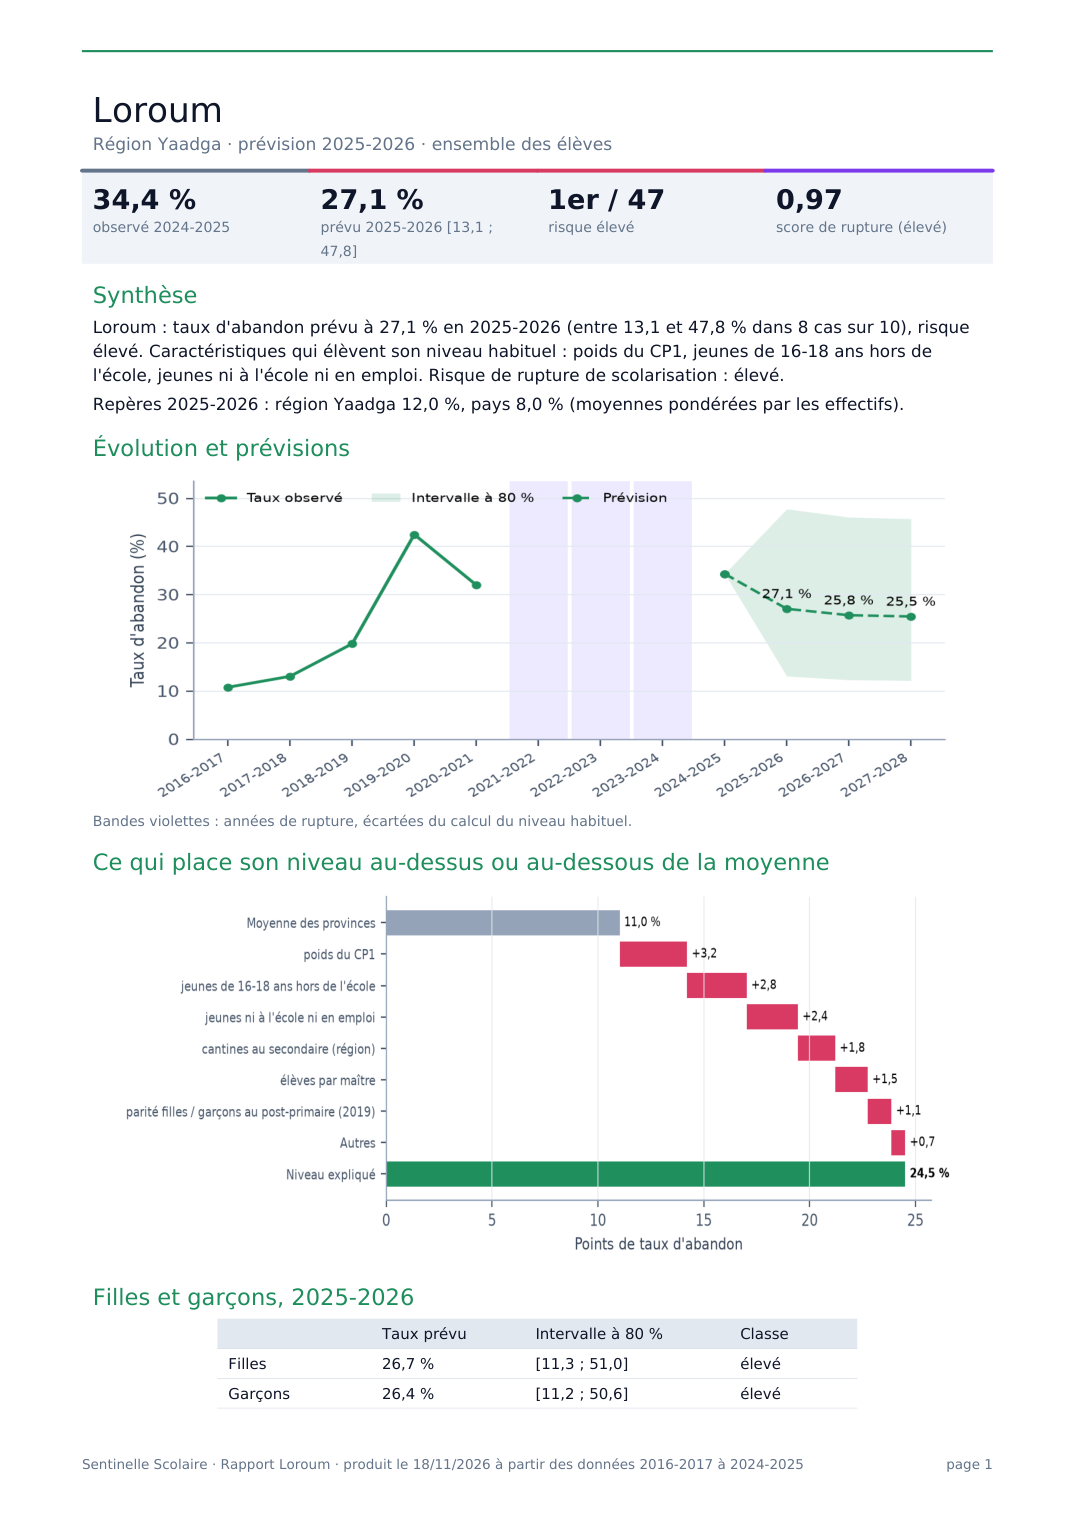
\includegraphics[width=0.475\textwidth]{fiche_loroum_p1}}\hfill
\fbox{
\includegraphics[width=0.475\textwidth]{fiche_loroum_p2}}
\caption{Exemple de livrable : la fiche de décision du Loroum, générée automatiquement (deux pages). Synthèse, repères région et pays, évolution et prévisions, facteurs, filles et garçons, risque de rupture, pistes d'action, méthode et sources.}
\label{fig:fiche}
\end{figure*}

\subsection{Impact}

Le ciblage est efficace. Les 12 provinces en risque élevé ne regroupent que 5,9 \% des élèves du primaire, mais environ 36\,200 des 266\,000 abandons attendus en 2025-2026. Les neuf provinces à la fois en risque élevé et en alerte de rupture (Loroum, Karo-Peli, Djelgodji, Séno, Yagha, Oudalan, Gobnangou, Dyamongou, Kompienga) comptent 100\,000 élèves et environ 21\,600 abandons attendus : c'est là qu'une action précoce, continuité éducative, suivi des élèves dès le CP1, seconde chance pour les adolescents, protège le plus d'enfants par franc dépensé. Les facteurs orientent ces leviers ; les provinces qui résistent indiquent où chercher des pratiques qui marchent ; le volume, enfin, indique où dimensionner les moyens.

\begin{table}[!htbp]
\centering
\footnotesize
\begin{tabularx}{\columnwidth}{@{}L{2.05cm} Y L{1.85cm}@{}}
\toprule
Facteur & Piste d'action & Indicateur à suivre \\
\midrule
Poids du CP1 & suivre chaque élève dès le CP1 (absences, redoublements), lecture dès la première année & rapport CM2/CP1 \\
Adolescents hors de l'école & passerelles de seconde chance, éducation non formelle & jeunes de 16-18 ans hors école \\
Jeunes sans école ni emploi & lier l'école aux programmes d'emploi et de formation & jeunes 15-24 ans ni école ni emploi \\
Élèves par maître & affecter des enseignants vers les classes surchargées & élèves par maître \\
Places assises manquantes & tables-bancs, salles de classe & places manquantes pour 100 élèves \\
Mariage précoce & prévention avec les leaders communautaires, maintien des filles & abandons pour mariage ou grossesse \\
Rupture probable & continuité éducative : écoles d'accueil, enseignement à distance, recensement des élèves déplacés & score de rupture, écoles fermées \\
\bottomrule
\end{tabularx}
\caption{Des facteurs aux actions : chaque facteur mis en évidence par le modèle oriente une piste et un indicateur de suivi. Ce sont des pistes à examiner avec les équipes, pas des effets garantis.}
\label{tab:actions}
\end{table}

Le tableau~\ref{tab:actions} relie chaque facteur à une piste d'action et à un indicateur que l'outil permet de suivre d'une année à l'autre ; les rapports régionaux et les fiches provinciales reprennent automatiquement les pistes liées aux facteurs de chaque territoire.

\subsection{Faisabilité}

\textbf{Pour l'administration}, l'outil ne demande ni serveur coûteux ni compétence rare. Il tourne hors ligne sur un ordinateur ordinaire ; en ligne, un hébergement de conteneurs coûte quelques dollars par mois. La mise à jour annuelle se fait en quelques minutes, sans réentraînement ; un réentraînement complet, tous les deux ou trois ans, consiste à relancer la chaîne documentée. \textbf{Les données} sont celles que la DGESS et l'INSD publient déjà : aucune collecte nouvelle n'est nécessaire. \textbf{La chaîne} compte environ 16\,500 lignes de code commenté, en modules par étape, avec des notebooks exécutés et des contrôles automatiques à chaque étape.

\subsection{Ce qui est nouveau}

\begin{table}[!t]
\centering
\footnotesize
\begin{tabularx}{\columnwidth}{@{}Y L{1.9cm}@{}}
\toprule
Innovation & État \\
\midrule
Séparer l'abandon et la rupture : deux modèles & livrée \\
Évaluation sur une année jamais vue, règle écrite à l'avance & livrée \\
Intervalles conformes à couverture vérifiée, entre 0 et 100 \% & livrée \\
Provinces qui résistent, mesurées sur des provinces non vues & livrée \\
Simulateur de leviers & livrée \\
Assistant qui cite ses sources, sur 64 indicateurs & livrée \\
Mise à jour annuelle sans réentraînement & livrée \\
Rapports PDF générés automatiquement & livrée \\
Rapport de qualité des données pour la DGESS & éléments livrés (journal, contrôles, statut des cellules) \\
Indice mensuel d'exposition aux fermetures d'écoles & suite prévue \\
\bottomrule
\end{tabularx}
\caption{Innovations de \sol{}.}
\label{tab:innovations}
\end{table}

Le tableau~\ref{tab:innovations} résume les innovations. La plus importante n'est pas technique : c'est \textbf{l'honnêteté de la prévision}. Plutôt que d'afficher un modèle complexe qui aurait gagné sur une année par chance, nous montrons qu'un modèle simple, bien évalué, avec une incertitude vérifiée, suffit à guider la décision, et nous l'outillons pour qu'il serve chaque année.

\subsection{Limites et suites}

Neuf années par province, c'est peu : les intervalles restent larges (18 à 20 points), et les projections au-delà de trois ans ne seraient pas validées, d'où l'horizon de 2027-2028. Les provinces créées en 2025 héritent de l'historique de leur province d'origine. Les facteurs et le simulateur décrivent des associations, pas des causes : une évaluation d'impact resterait nécessaire avant de généraliser une mesure. Le nombre d'élèves qui abandonnent suppose des effectifs constants. Deux suites sont prévues : un rapport de qualité des données pour la DGESS, à partir du journal de nettoyage, des contrôles et du statut de chaque cellule, et un indice mensuel d'exposition aux fermetures d'écoles tiré des rapports du ST-ESU, pour alerter avant la sortie de l'annuaire.

%======================================================================
\section{La reproduction}
%======================================================================

\textbf{Utiliser l'outil.} En ligne : \lien. Sur un ordinateur Windows, sans Internet : \texttt{application/lancer.bat}. Sur toute machine avec Docker : \texttt{docker compose up --build} dans \texttt{application/}.

\textbf{Relancer la chaîne.} Python 3.13 ou plus récent, \texttt{pip install -r requirements.txt}, puis, avec \texttt{src} dans le chemin Python, dans cet ordre : \texttt{sentinelle.collecte}, \texttt{.nettoyage}, \texttt{.transformation}, \texttt{.apurement}, \texttt{.analyse}, \texttt{.interpretation} (une commande \texttt{python -m} par étape). Chaque commande régénère ses sorties et son dépôt, et 15 tests automatiques (	exttt{python -m pytest}) vérifient les calculs clés, la cohérence entre l'analyse et l'application et la reproduction exacte des prévisions par la mise à jour annuelle ; les notebooks \texttt{01} à \texttt{04c}, exécutés, présentent chaque étape. Les modèles retenus sont sauvegardés avec une fiche (\texttt{fiche\_modele.json}) qui donne les réglages, les marges, les seuils, la qualité mesurée et les versions des bibliothèques.

\begin{table}[!t]
\centering
\footnotesize
\begin{tabularx}{\columnwidth}{@{}L{2.05cm} r Y@{}}
\toprule
Dépôt & Fichiers & Rôles et contenu \\
\midrule
01\_collecte & 53 & engineer : extractions brutes, registre et bilan des sources, inventaire \\
02\_nettoyage & 43 & engineer, architect : tables propres, journal, contrôles, base GeoPackage, dictionnaire, document technique \\
03\_transformation & 27 & engineer, architect : table d'analyse, base apurée, schéma, métadonnées, plan du parcours, document technique \\
04\_analyse & 70 & analyst, scientist : exploration, prévisions, fiabilité, modèles et leur fiche, SHAP, alerte, code, notebooks \\
05\_interpretation & 10 & analyst : documentation, indicateurs clés, carte d'alerte, rapports, guide, code du tableau de bord \\
\bottomrule
\end{tabularx}
\caption{Dépôts de l'équipe, nommés \texttt{DiscernaTeam\_ÉTAPE\_D1\_RÔLE\_description\_vN}, chacun avec son LISEZ-MOI.}
\label{tab:depots}
\end{table}

\textbf{Dépôts et documents techniques.} Les 203 fichiers déposés suivent la convention du challenge et chaque dépôt contient un fichier LISEZ-MOI (tableau~\ref{tab:depots}). Le détail de la collecte et du nettoyage, et celui du passage au découpage de 2025, sont décrits dans deux documents techniques déposés avec les étapes 02 et 03 ; le code du modèle et ses notebooks sont déposés avec l'étape 04, et le code du tableau de bord avec l'étape 05.

\FloatBarrier
\bibliographystyle{named}
\bibliography{references}

\end{document}
